\documentclass[12pt]{article}

% Page layout
\usepackage[margin=1in]{geometry}
\PassOptionsToPackage{table,xcdraw}{xcolor}

% Math
\usepackage{amsmath}
\usepackage{amsfonts}
\usepackage{amsthm}
\usepackage{siunitx}
\usepackage{threeparttable}

% Graphics and floats
\usepackage{graphicx}
\usepackage{subcaption}
\usepackage{float}
\usepackage{adjustbox}
\usepackage{makecell}
\usepackage{tikz}
\usetikzlibrary{shapes.geometric, arrows.meta, positioning, fit, backgrounds}
\usetikzlibrary{calc}
\usepackage{chessfss}
\usepackage[OT1]{fontenc}
% Tables
\usepackage{booktabs}
\usepackage{multirow}
\usepackage{diagbox}
\usepackage{listings}
\usepackage{tabularx}
\usepackage{xcolor}
\usepackage{booktabs}

\usepackage{listings}
\usepackage{xcolor}

\lstset{
    basicstyle=\ttfamily\small,
    backgroundcolor=\color{yellow!3!white},
    breakatwhitespace=true,
    breaklines=true,
    columns=fullflexible,
    commentstyle=\color{red!70!black},
    frame=single,
    framerule=1pt,
    identifierstyle=\color{green!40!black},
    keywordstyle=\bfseries\color{blue!80!black},
    numbers=left,
    numbersep=8pt,
    numberstyle=\scriptsize\sffamily\itshape\color{black!80},
    rulecolor=\color{blue!70!black},
    rulesepcolor=\color{blue!30!black},
    showstringspaces=false,
    stringstyle=\color{orange},
    tabsize=4,
    xleftmargin=15pt,
    xrightmargin=15pt,
    resetmargins=true,
}

% Text formatting
\usepackage[normalem]{ulem}
\useunder{\uline}{\ul}{}
\usepackage{titlesec}
\usepackage{verbatim}

% Hyperlinks
\definecolor{darkgreen}{rgb}{0.0, 0.5, 0.0}
\usepackage[colorlinks=true, linkcolor=blue, citecolor=darkgreen]{hyperref}
\usepackage[font=small]{caption}

% Custom itemize environment
\newenvironment{packed_item}{
\begin{itemize}
  \setlength{\itemsep}{1pt}
  \setlength{\parskip}{0pt}
  \setlength{\parsep}{0pt}
}{\end{itemize}}

% Custom float centering
\makeatletter
\newcommand*{\centerfloat}{%
  \parindent \z@
  \leftskip \z@ \@plus 1fil \@minus \textwidth
  \rightskip\leftskip
  \parfillskip \z@skip}
\makeatother

\newcommand{\m}[1]{\mathbf{#1}}
% Section formatting
\setcounter{secnumdepth}{4}
\titleformat{\paragraph}
{\normalfont\normalsize\bfseries}{\theparagraph}{1em}{}
\titlespacing*{\paragraph}
{0pt}{2ex plus 1ex minus .5ex}{2ex plus .5ex}


\setlength{\parindent}{0.4in}

\begin{document}
\title{Optimizing AI Tutoring Design for Learning and Engagement: A Response Surface Methodology Study}
\author{Shivsai Sharda}
\date{\today}
\maketitle
\tableofcontents
\newpage

\section{Introduction}
\subsection{Key Terms}
The following terms are important to this paper.
\begin{itemize}
    \item \textbf{Testing Performance/Achievement:} The ability to perform on standardized testing. This is often a measure of a student's ability to retain and acquire information related to the topic being tested, but may be slightly influenced by factors such as test-taking ability, assessment design, and inherent motivation.
    \item \textbf{Independent Reasoning Capacity (IRC):} The ability to independently evaluate information, generate defensible conclusions, and assess one's own learning. This is an aggregate of several different metrics, which are presented in Table $\ref{tab:zimmerman_mapping}$.
\end{itemize}
\subsection{Problem \& Consequences}
Benjamin Bloom's 1984 paper introduced the 2 Sigma Problem \cite{bloom1984sigma} --- the finding that 1-on-1 tutoring could propel a student's testing performance nearly two standard deviations\footnote{This number is heavily debated in the education community, in large part due to the study referred to in Bloom's paper engaging participants with concepts they had never encountered before, leading to the large positive effect from 1:1 tutoring. However, experts maintain that 1:1 tutoring indeed has a moderate-significant positive effect in comparison to classroom instruction.} higher, but that 1:1 tutoring was not scalable. Ever since, personalized tutoring has been referred to as the gold standard; Mark Zuckerberg, for instance, has invested \$45 billion USD through the Chan Zuckerberg Initiative \cite{kim2016zuckerberg}. Microsoft, Google, and other corporations have made similar multimillion-dollar investments in personalized learning \cite{beatty2024khanmicrosoft, googlecloud_learnlm}.
\\\\
While the issue of non-scalability stands, students remain at an academic level lower than what is theoretically achievable. Standardized assessments persist as key metrics for measuring academic achievement. Tens of billions of dollars of federal funding are being invested yearly into improving student results in standardized testing \cite{ed2021budgethistorytable}. Yet despite the funding being funneled into this sector, average NAEP\footnote{National Assessment of Educational Progress, often referred to as the Nation's Report Card.} scores decreased from $243$ in 2012 to $241$ in 2020 (Figure \ref{fig1}) \cite{naep2025math9}. Had personalized learning been possible in 2012, a $2 \sigma$ increase in performance would instead have placed the average student well over the 90th percentile, with average scores over $286$. These statistics suggest that personalized learning is a promising approach to better test scores.
\begin{figure}[!ht]
    \centering
    \includegraphics[width=1\linewidth]{naep.png}
    \caption{NAEP long-term mathematics trend scores for 9-year-old students with current structure \cite{naep2025math9}}
    \label{fig1}
\end{figure}
\\\\
The effects of stunted academic performance will become apparent on the individual and community level as well. One severe detrimental consequence will be the ease to spread misinformation. A study run by Shaw and Nave demonstrated that participants trusted faulty AI responses $79.8\%$ of the time, with $11.7 \%$ more confidence than other participants answering the same questions without AI access \cite{shaw2026thinking}. Especially with only $70\%$ of 12th graders demonstrating grade-level competency ($\ge$ NAEP Basic) on the NAEP Reading portion \cite{naep2023reading12}, this leaves $30 \%$ of the population especially vulnerable to misinformation because they lack much of the knowledge necessary to fact-check it. Misinformation will only become more prevalent, with the rise of political deepfakes \cite{dale2026talarico} and hyper-targeted advertisements designed specifically to match the viewer's identity, thoughts, and beliefs. The inability to identify this, a result of limited media literacy, could have consequences in elections and law and related fields. 


\subsubsection{Non-AI (Traditional) Approaches}\label{fail}

It is infeasible for school districts to scale tutoring in the traditional way. Because one human tutor would be required per student, the cost of hiring teachers grows linearly with the number of students, and spending nearly $75,000$ USD per student is infeasible.
\\\\
Moreover, designing a deterministic intelligent tutoring system (ITS) fails to provide the $2\sigma$ improvement from Bloom's paper \cite{bloom1984sigma}. An ITS is a pedagogically-designed computer application to scaffold learning. There are several reasons for this:
\begin{itemize}
    \item An ITS cannot respond to natural language prompts, since its interactions are limited to pre-scripted messages.
    \item A student cannot ask questions of the ITS, so it fails to clear up confusion.
    \item A unique solution pathway constructed by the student may not have been coded into the ITS, causing the ITS to falsely convey that the student's method is incorrect.
\end{itemize}
To make it concrete, the leading ITS --- \emph{Carnegie Learning's Cognitive Tutor} --- resulted in $.29 \sigma \ll 2 \sigma$ growth in performance in an RCT \cite{jaciw2007cognitivetutor}.

\subsection{Literature Review}
From Section $\ref{fail}$, we can conclude that a tool that supports both NLP and has a reasonable cost is necessary. LLMs satisfy both constraints --- they are designed to handle natural language, and can work at negligible costs relative to human tutors.
\\\\
However, using LLMs to drive scalability comes with a hidden cost. Pedagogy has demonstrated the somewhat paradoxical nature of learning: the more seamless the learning process is, the less knowledge retained by the student \cite{bjork2011making}. Not only does it prevent long-term knowledge retention, but it also hinders the growth of one's independent reasoning. However, with common LLMs such as ChatGPT or Claude, the process is so fluid that students are able to offload the entirety of their cognitive effort to the AI system.\footnote{This is in fact a design choice. LLMs aim to enhance productivity and efficiency, as that is desirable in the \textbf{workplace}. But this efficiency comes with a cognitive cost; one that is acceptable in the workplace, but detrimental in education. For the purposes of an analogy, consider a 2nd grader learning arithmetic. Access to a calculator would allow them to circumvent the process of learning fundamental skills, such as adding two digit numbers. However, for a high schooler, using a calculator is fair game and is even encouraged.} An MIT Media Lab study demonstrated that using an LLM when completing a task causes a significant drop in brain connectivity, providing another reason behind limited recall \cite{kosmyna2025brainchatgptaccumulationcognitive}.

\begin{figure}[h]
\begin{minipage}{0.5\textwidth}
    \centering
    \includegraphics[width=1\linewidth]{claudesolve.png}
    \caption{Claude Solving a Math Problem}
    \label{fig:myimage}
\end{minipage}
\hfill
\begin{minipage}{0.5\textwidth}
    \begin{center}
    \textbf{Pedagogical Issues with Claude's Response.}
    \end{center}
    \begin{itemize}
        \item Provides the solution in seconds, requiring no analysis from the student.
        \item Provides entire solutions, even when asked to ``help" the student with their work.
        \item Provides assistance upon request.
    \end{itemize}
\end{minipage}
\end{figure}

 Bastani et al.'s RCT demonstrated this effect empirically --- unrestricted AI access in high school students caused a $17\%$ decline in exam performance relative to students without access\footnote{The tutoring system in the paper uses the GPT 4 API Key; the paper establishes that the model provides the wrong answer $51\%$ of the time. This could definitely inflate the decline amount; however, a large inflation in the decline amount would demonstrate that students did not critically think about AI responses.}, whereas safeguarded AI produced no change in exam performance \cite{doi:10.1073/pnas.2422633122}. These findings demonstrate that plain LLM usage provides \emph{no non-trivial advantage} over standard 1-to-many instruction when measured by academic performance.
 \\\\
 To see the effect of LLMs on independent reasoning capacity (IRC), we divide IRC into three measurable components:
 \begin{itemize}
     \item \textbf{Metacognitive Calibration.} To what extent does a student's knowledge of a subject align with their perceived knowledge?
     \item \textbf{Transfer Performance.} How well can a student apply knowledge to problems structurally different from those practiced?
     \item \textbf{Initiation Tendency.} How readily does a student attempt problems independently before offloading cognitive work to an AI model or a secondary person?
 \end{itemize}

This construct of independent reasoning capacity aligns with Zimmerman's qualities of a self-regulating learner \cite{Zimmerman2000}.

\begin{table}[H]
\centering
\caption{IRC to Zimmerman Mapping}
\label{tab:zimmerman_mapping}
\renewcommand{\arraystretch}{1.2}
\begin{tabular}{p{0.30\linewidth} p{0.62\linewidth}}
\toprule
\textbf{IRC Facet} & \textbf{Zimmerman Alignment} \\
\midrule
Metacognitive Calibration &
\textbf{Self-reflection:} Self-evaluation and causal attribution following an assessment \cite{Zimmerman2000}. \\
\midrule
Initiation Tendency &
\textbf{Forethought:} Intrinsic interest and learning goal orientation: valuing the problem-solving \textbf{process} \cite{Zimmerman2000}. \\
\midrule
Transfer Performance &
\textbf{Performance, Forethought:} Developing adaptable strategies to attempt unfamiliar problems \cite{Zimmerman2000}. \\
\bottomrule
\end{tabular}
\end{table}

Although this division of IRC may not be exhaustive, these components were chosen due to their measurability. The key point is that, just as standard LLMs hurt long-term knowledge retention, they negatively affect IRC as well. In Bastani's RCT, students with access to LLMs during practice sessions reported feeling more confident in their knowledge of the material compared to their peers, but performed worse or at par with them on assessments \cite{doi:10.1073/pnas.2422633122}, demonstrating a drop in metacognitive calibration. Moreover, the same study shows that students using GPT Base, the standard GPT-4 API, began to ask for answers on the first message more frequently over the sessions, with $29\%$ of first messages asking for the answer in Session 1 and $36\%$ of first messages asking for the answer in Session 4. Although the shift is faint, it indicates that LLMs downgrade a student's initiation tendency \cite{doi:10.1073/pnas.2422633122}. Finally, depth and nuance are critical for developing transferable knowledge, and AI eliminates both in order to simplify its prose \cite{Vendrell2026Scaffolding}.
\\\\
As a result, it is imperative that we alter standard LLMs in order to preserve both knowledge and IRC. The parameters we change here come from Vendrell and Johnston's 2026 framework on the $8$ principles to preserve critical thinking in the presence of AI \cite{Vendrell2026Scaffolding}. More specifically, we choose to alter:
\begin{itemize}
\item \textbf{Answer Specificity:} How much of the solution do successive hints give away?
\item \textbf{Access Delay:} How long is the forced wait before the AI responds, during which students must reason independently?
\item \textbf{Metacognitive Prompting Rate:} How frequently does the student receive a metacognitive prompt, that is, a prompt that forces them to think about their own work (for example, ``How confident are you in this step?'')?
\item \textbf{Scaffolding Fade Rate:} At what rate does AI assistance decline as a student improves?
\end{itemize}
We now bring in another key factor: engagement. Notice that our prior goal had been to maximize IRC and knowledge, and thus we chose the above parameters. But trivially maximizing each of the parameters maximizes IRC at the cost of suboptimal engagement. To see why empirically, we study Khanmigo.\footnote{Khan Academy's AI Tutor} Khanmigo was developed as a Socratic tutor, which means that it only questioned the learner to advance their knowledge \cite{khan2023harnessing}. This implies that Khanmigo did not give hints, thus sitting at a maximum for both answer specificity and access delay. As a result, only $15\%$ of students with access to Khanmigo used it beyond the weekly recommended amount --- a mere 30 minutes \cite{khanacademy2026learninginopen}. Yet, as expected, Khanmigo produced excellent achievement results in the schools that did use it actively \cite{oreopoulos2026khanacademy}.
\\\\
Existing AI tutoring systems, to our knowledge, sit at one of two extremes on these parameters: either the parameters are applied at full strength or they are absent entirely, as in a standard conversational assistant. We are not aware of a system that has been deployed at an intermediate setting, nor of work characterizing what should happen in between. This is the gap the present study addresses.
\subsection{Research Approach}

The research question explored in this paper is:

\begin{quote}
    At what combination of the aforementioned parameters does an AI tutoring system provide sufficient support and engagement for the learner and improve performance, while enhancing their independent reasoning skills?
\end{quote}

\noindent Here, independent reasoning is measured by the metrics above. This question addresses the gap left by other tutoring systems, which fail to account for learner engagement. Engagement is crucial: without it, the tool cannot enhance a student's IRC, because the student will not use the tool at all. An AI analytics study by UPenn Wharton finds that engagement, rather than content, is often the factor that drives the most improvement \cite{wharton}. By creating this tool, we design the foundation for a system that students will actually use for learning. This will lead to increases in performance, as desired by the U.S. Department of Education \cite{usdoe2015essa}, but will also increase independent reasoning, a highly valuable trait \cite{wef2025futureofjobs}.

\subsubsection{Theory of Change}

This work establishes the foundation for a good tutoring system, not the system itself: parameters alone would produce better engagement than existing tools, but insufficient for students to return to it without additional layers of design. One such layer consists of several cosmetic changes to make it more accessible and student-friendly, but the most important layer is one that makes the AI tool \emph{proactive}, rather than reactive \cite{wharton}.
\\\\
With these modifications complete, the tutoring system should function as intended and prove effective in the desired areas. The last bottleneck is deploying it into classrooms nationally. To accomplish this, it would be best to partner with a popular, renowned edtech company (e.g., Khan Academy, Instructure) to facilitate distribution. We recognize that this will be a difficult process, but it is worth attempting. Home use would also be valuable, but the theory of change there is more complicated, since students have far more agency outside the classroom. At home they already have access to the most engaging general-purpose LLMs, such as Claude and ChatGPT, which makes switching them to a pedagogical tutor significantly more difficult. This study therefore prioritizes classroom deployment as teachers have more direct influence there, and students tend to carry classroom practices home once those practices have paid off for them. We elaborate more on the theory of change in the flowchart on the next page.

\paragraph{Failure Modes / Assumptions}
In the following flowchart, we expect the first three stages (up to Enhancement \#2) to proceed smoothly. Most of the design work behind the enhancements has already been done, and it is just a matter of integrating it well. The primary difficulty arises from partnering with edtech companies, as the product will not have ``real-world testing'' beyond this paper. Direct-to-school outreach is also difficult, as districts prefer to collaborate with edtech companies instead. However, more research and testing can make such partnerships possible. Another point of difficulty will be motivating students to use the system at home. However, once the system has been released for a while and its benefits are known, this should resolve itself.


\begin{figure}[p]
\centering
\resizebox{\textwidth}{!}{%
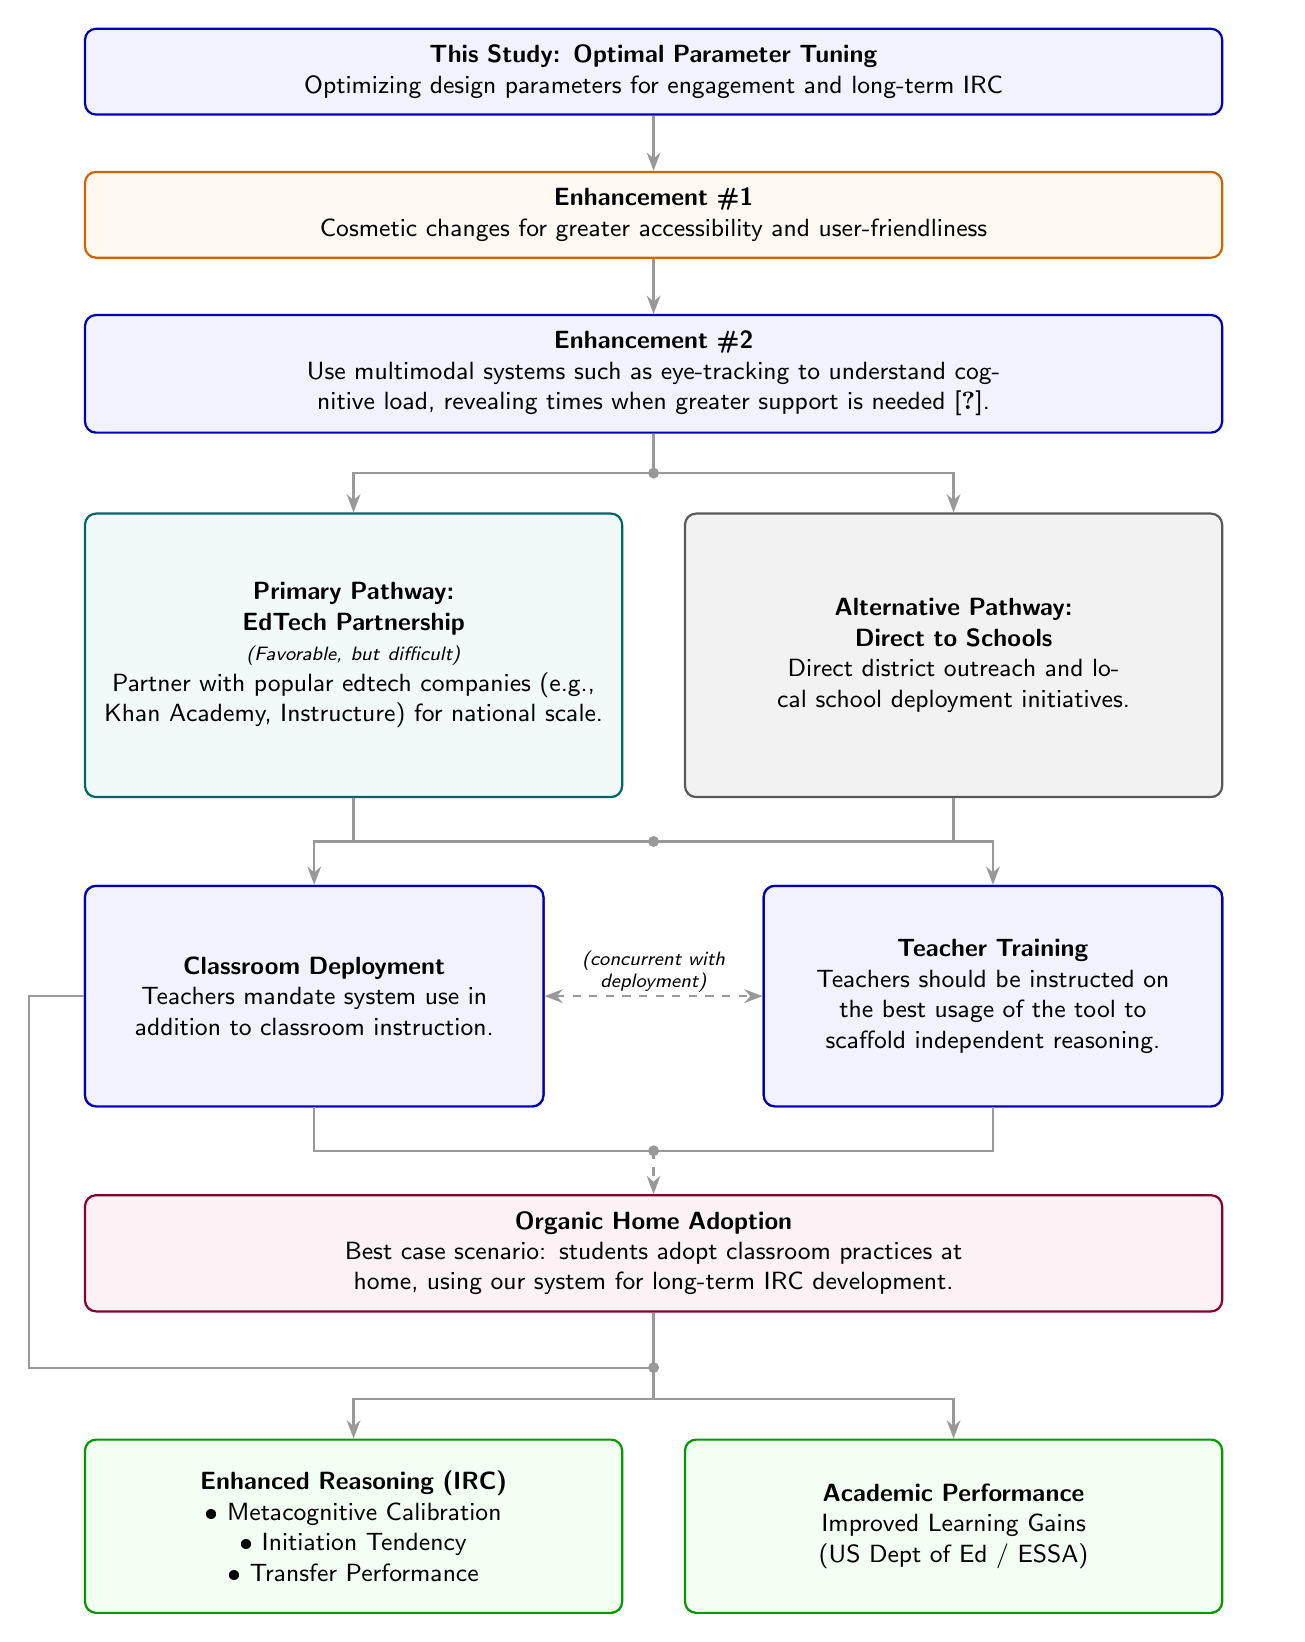
\begin{tikzpicture}[
    font=\sffamily\small,
    % Styles
    block/.style={rectangle, draw=blue!70!black, fill=blue!5, thick, rounded corners,
                  align=center, inner sep=6pt, text width=14.02cm},
    layer/.style={rectangle, draw=orange!80!black, fill=orange!5, thick, rounded corners,
                  align=center, inner sep=6pt, text width=14.02cm},
    home/.style={rectangle, draw=purple!70!black, fill=purple!5, thick, rounded corners,
                  align=center, inner sep=6pt, text width=14.02cm},
    pathprimary/.style={rectangle, draw=teal!80!black, fill=teal!5, thick, rounded corners,
                  align=center, inner sep=6pt, text width=6.4cm, minimum height=3.6cm},
    pathalt/.style={rectangle, draw=gray!70!black, fill=gray!10, thick, rounded corners,
                  align=center, inner sep=6pt, text width=6.4cm, minimum height=3.6cm},
    deploy/.style={rectangle, draw=blue!70!black, fill=blue!5, thick, rounded corners,
                  align=center, inner sep=6pt, text width=5.4cm, minimum height=2.8cm},
    outcome/.style={rectangle, draw=green!60!black, fill=green!5, thick, rounded corners,
                  align=center, inner sep=6pt, text width=6.4cm, minimum height=2.2cm},
    arrow/.style={-Stealth, thick, draw=gray!80},
    dashedarrow/.style={-Stealth, thick, dashed, draw=gray!80},
    line/.style={thick, draw=gray!80},
    dot/.style={circle, fill=gray!80, inner sep=1.4pt}
]

    % ---------- Trunk ----------
    \node (params) [block] {
        \textbf{This Study: Optimal Parameter Tuning}\\
        Optimizing design parameters for engagement and long-term IRC
    };

    \node (layer1) [layer, below=0.7cm of params] {
        \textbf{Enhancement \#1}\\
        Cosmetic changes for greater accessibility and user-friendliness
    };

    \node (layer2) [block, below=0.7cm of layer1] {
        \textbf{Enhancement \#2}\\
        Use multimodal systems such as eye-tracking to understand cognitive load, revealing times when greater support is needed \cite{mueller2026eyets}.
    };

    % ---------- Fork: adoption pathways ----------
    \node (edtech) [pathprimary, anchor=north] at ($(layer2.south)+(-3.81,-1.0)$) {
        \textbf{Primary Pathway:}\\
        \textbf{EdTech Partnership}\\
        \textit{\scriptsize (Favorable, but difficult)}\\
        Partner with popular edtech companies (e.g., Khan Academy, Instructure) for national scale.
    };

    \node (direct) [pathalt, anchor=north] at ($(layer2.south)+(3.81,-1.0)$) {
        \textbf{Alternative Pathway:}\\
        \textbf{Direct to Schools}\\
        Direct district outreach and local school deployment initiatives.
    };
    \coordinate (pairtop) at ($(edtech.south)+(3.81,-1.1)$);

    \node (classroom) [deploy, anchor=north] at ($(pairtop)+(-4.31,0)$) { ... };
    \node (hello)     [deploy, anchor=north] at ($(pairtop)+(4.31,0)$)  { ... };
    % ---------- Concurrent pair ----------
    \node (classroom) [deploy, anchor=north] at ($(edtech.south)+(-0.50,-1.1)$) {
        \textbf{Classroom Deployment}\\
        Teachers mandate system use in addition to classroom instruction. 
    };

    \node (hello) [deploy, anchor=north] at ($(direct.south)+(0.50,-1.1)$) {
        \textbf{Teacher Training}\\
        Teachers should be instructed on the best usage of the tool to scaffold independent reasoning.
    };

    % ---------- Home adoption ----------
    \node (home) [home, anchor=north] at ($(classroom.south)+(4.31,-1.1)$) {
        \textbf{Organic Home Adoption}\\
        Best case scenario: students adopt classroom practices at home, using our system for long-term IRC development.
    };

    % ---------- Junctions ----------
    \coordinate (fork)     at ($(layer2.south)+(0,-0.5)$);
    \coordinate (jointop)  at ($(edtech.south)+(3.81,-0.55)$);
    \coordinate (pairjoin) at ($(classroom.south)+(4.31,-0.55)$);
    \coordinate (merge)    at ($(home.south)+(0,-0.7)$);
    \coordinate (split)    at ($(merge)+(0,-0.4)$);

    % ---------- Outcomes ----------
    \node (irc) [outcome, anchor=north] at ($(split)+(-3.81,-0.5)$) {
        \textbf{Enhanced Reasoning (IRC)}\\
        \textbullet{} Metacognitive Calibration\\
        \textbullet{} Initiation Tendency\\
        \textbullet{} Transfer Performance
    };

    \node (perf) [outcome, anchor=north] at ($(split)+(3.81,-0.5)$) {
        \textbf{Academic Performance}\\
        Improved Learning Gains\\
        (US Dept of Ed / ESSA)
    };

    % ---------- Connections ----------
    \draw [arrow] (params) -- (layer1);
    \draw [arrow] (layer1) -- (layer2);

    % split into the two adoption pathways
    \draw [line]  (layer2.south) -- (fork);
    \node [dot] at (fork) {};
    \draw [arrow] (fork) -| (edtech.north);
    \draw [arrow] (fork) -| (direct.north);

    % pathways re-converge, then feed the concurrent pair
    \draw [line]  (edtech.south) |- (jointop);
    \draw [line]  (direct.south) |- (jointop);
    \node [dot] at (jointop) {};
    \draw [arrow] (jointop) -| (classroom.north);
    \draw [arrow] (jointop) -| (hello.north);

    % concurrency link, labelled above the arrow
    \draw [Stealth-Stealth, thick, dashed, draw=gray!80]
          (classroom.east) -- (hello.west)
          node [midway, above, inner sep=1pt, text width=2.4cm, align=center,
                font=\sffamily\scriptsize]
               {\textit{(concurrent with\\ deployment)}};

    % pair -> home adoption
    \draw [line] (classroom.south) |- (pairjoin);
    \draw [line] (hello.south)     |- (pairjoin);
    \node [dot] at (pairjoin) {};
    \draw [dashedarrow] (pairjoin) -- (home.north);

    % deployment bypasses home and rejoins at the outcome junction
    \draw [line] (classroom.west) -- ++(-0.7,0) |- (merge);
    \draw [line] (home.south) -- (merge);
    \node [dot] at (merge) {};

    \draw [line]  (merge) -- (split);
    \draw [arrow] (split) -| (irc.north);
    \draw [arrow] (split) -| (perf.north);

    % balances the bounding box against the left-margin bypass
    \path (7.92,0);

\end{tikzpicture}%
}
\caption{\textbf{Theory of Change}}
\label{fig:theory_of_change}
\end{figure}

\newpage

\section{Methodology}

\textit{High-Level Summary.} Say we compress the input variables (answer specificity, access delay, etc.) into a column vector $\mathbf{x}$. Using a response surface methodology (RSM) approach, we develop one function per outcome (Table \ref{oink}) that maps the input parameters to five learning outcomes. We collect data for these functions through an experiment in which each student is assigned a design point and tutored by a system configured to that point. The composite learning outcome is modeled as a weighted sum
\[
c(\mathbf{x})=0.3 f(\mathbf{x})+0.2 g(\mathbf{x})+0.1 h(\mathbf{x}) + 0.4 p(\mathbf{x})
\]
Then the resulting problem is to maximize \(c(\mathbf{x})\) subject to the engagement constraint
\[
e(\mathbf{x})\ge e_{th},
\]
where \(e_{th}\) denotes the minimum acceptable engagement level for a given student. Here, $c(\mathbf{x})$ consists of both IRC and performance, a specific design decision elaborated on in Section \ref{sec3}.

\begin{table}[h]
\centering
\begin{tabular}{@{}llc@{}}
\toprule
Function & Outcome & Weight \\
\midrule
$f(\mathbf{x})$ & metacognitive calibration & $.3$ \\
$g(\mathbf{x})$ & transfer performance      & $.2$ \\
$h(\mathbf{x})$ & initiation tendency       & $.1$ \\
$p(\mathbf{x})$ & achievement (performance) & $.4$\\
$e(\mathbf{x})$ & engagement                & -- \\
\bottomrule
\end{tabular}
\caption{Each response function maps $\mathbf{x}$ to one learning
outcome.}
\label{oink}
\end{table}

\paragraph{RSM Background}

This section is primarily deferred to the appendix due to a high technical bar. At a high-level, we use a second-order RSM approach to develop the function $f, g, h, p, e$. This allows us to take into account scenarios in which the input parameters interact with each other (e.g., the effect of one depends on another). Moreover, we use a central composite design (CCD), which requires $25$ unique data points, namely axial, factorial, and the center point.
\subsection{Study Design and Experimental Procedure}

To gather the necessary data for RSM, we conducted an experiment to understand how each set of parameters correlates with each of the outputs. We collaborated with a primary school in an Indian suburb, which provided a strong baseline control\footnote{Though this did come with several downsides: students did not understand what the tool was at the beginning and spent a considerable amount of time simply testing it out.} as students had minimal prior exposure to AI tools. Approximately $N=100$ students were assigned a random \texttt{condition\_slot} that corresponds to a data point needed for the RSM model, and were asked to use the system for $10$ hours. However, only $32$ used it.
\\\\
During the experiment, students interacted with an AI tutoring system specifically designed to follow the input parameters. At the beginning, they also responded to a survey to help understand their prior mathematical ability and level of engagement with mathematics. Students were aware that there were constraints placed on the tutor, but did not know the exact parameters assigned to their model beyond the access delay. Students did, however, know when they were in a delay period and whether they could ask for a hint.
\\\\
The AI tutoring system used the GPT-4 mini API for conversation, but used the o3 model when internally solving problems. We chose GPT-4 mini due to cost limitations; other frontier models cost several times more and would have been prohibitively expensive. However, due to GPT-4 mini's observed inability to solve complex\footnote{In fact, it sometimes could not solve simple math problems such as $x^2+x-10=0$. This was a large pain point.} math problems, it was necessary to use a stronger model for reasoning tasks such as solution generation. The o3 solution was then used by GPT-4 mini to guide answer validation and the hint pathway, neither of which required extra reasoning. This aligned with Bastani et al.'s design for their GPT tutor, in which (human) teachers provided solutions to prevent hallucination \cite{bastaniharm}.
\\\\
Interactions between the student and the AI system were restricted to math only. Students were allowed to ask for help on problems and on learning topics; for the latter, the parameters (e.g., access delay) were not relevant and students could receive instruction at any time. Every $2$ hours of interaction, students were required to take an assessment in order to continue with the study. Each assessment contained $10$ problems, distributed roughly as $7$ performance problems and $3$ transfer problems. Students were given $30$ minutes to complete each assessment, as the problems were AI-generated and thus easier than normal. The assessment problems were based on problems completed during practice. After each assessment, students had to predict their score on the assessment, as well as rate their learning and the difficulty of the test. The former helps compute metacognitive calibration, whereas the latter two help identify anomalies within the data.
\\\\
A major part of developing the application upon which the experiment was conducted was ensuring that the AI tutoring system adhered to the parameters. To achieve this, we had a thorough system prompt, which can be found in Appendix A. 


\subsection{Parametrization of the Input}

We established that the input parameters are answer specificity, access delay, metacognitive prompting rate, and scaffolding fade rate. We now elaborate on the settings of these parameters used for our CCD model and experiment. Because the coded variable is always $x_i \in \{-2, -1, 0, 1, 2\}$, we use $\xi _i$ to represent what the variable means in reality.
\begin{table}[h]
    \centering
    \begin{tabular}{c|c|c}
    \toprule
        \text{Name}  & \text{Coded} & \text{Reality}  \\
    \midrule
        \text{Answer Specificity} (AS)   & $x_1$ & $\xi_1$ \\
    \midrule
        \text{Access Delay}  (AD)  & $x_2$ & $\xi_2$ \\
    \midrule
        \text{Metacognitive Prompting Rate}  (MCP)  & $x_3$ & $\xi_3$ \\
    \midrule
        \text{Scaffolding Fade Rate} (SFR)  & $x_4$ & $\xi_4$ \\
    \bottomrule
    \end{tabular}
    \caption{Code vs Reality}
    \label{tab:placeholder}
\end{table}
\\\\
\textbf{Answer Specificity.}  
Answer specificity refers to the rough percentage of the solution given away when the student is stuck or asks for a hint. Answer specificity is additive: if the previous hint gave away $p\%$ of the solution, the subsequent hint will give away $(p + \xi_1)\%$. Moreover, the answer to a problem is never given away, even if a hint is meant to give away $\ge 100\%$ of the solution; this ensures that at least minimal cognitive effort is applied. To convert from coded units to actual (so-called ``natural'') units, we use the formula
\[\xi_1 = 12x_1 +30.\] Given that the coded units are points where $x_1 \in \{-2, -1, 0, 1, 2\}$, the natural values are $\xi_1 \in \{6, 18, 30, 42, 54\}$. These specific values were chosen with the assumption that practice problems take roughly $3$ steps, which is why $x_1=0 \implies \xi_1 = 30$. One key limitation of this structuring is that the latter $3$ values in the set, specifically $30, 42,$ and $54$, correspond to $2$--$4$ hints, whereas $\xi_1 = 6$ corresponds to $16$ hints. However, this is bound to happen with any choice of mapping from $x_1$ to $\xi_1$, because the number of hints is $100/\xi_1$, which grows rapidly. In order to enforce these parameters, the AI system was given a prompt isomorphic to
\begin{enumerate}
    \item Write out the solution to the problem. Break up the solution into the smallest chunks possible that still require cognitive effort and are not simple computations.
    \item Assign a percentage to each step from above describing how much of the solution it gives away. These percentages must sum to 100.
    \item The hint should consist of the next $n$ steps (adding on to the previous hint and the student's work) such that the sum of the percentages associated with those steps is as close as possible to $\xi_1$.
\end{enumerate}
This reveals another limitation, specifically that the exact $\xi_1$ cannot be followed most of the time. However, we make the best effort to follow $\xi_1$ without having to give useless hints.
\\\\
\textbf{Access Delay.} Access delay refers to the forced time in which the user attempts the problem without AI assistance. This occurs both at the beginning of the problem and between hints. In accordance with Kapur's productive failure framework, the period of access delay is significantly longer at the beginning of the problem than during it. Here, we use the formula
\[\xi_2 = 70 \cdot 3^{x_2/4}.\] This provides the conversion
\[\{-2, -1, 0, 1, 2\} \longrightarrow \{40, 53, 70, 92, 121\},\] where the values in the second set have been rounded to the nearest integer. We still need to take into account the difficulty of the problem. Clearly, an easier problem for the learner should not receive the same access delay as one that is extremely hard for the learner. Letting the difficulty of the problem be a variable $d \in \{1,\dots, 5\}$, the delays are given by
\[\text{initial access delay} = \xi_2 \cdot  3^{(d-1)/4}\]
\[\text{mid-problem access delay} = \frac {\xi_2}{2} \cdot 3^{(d-1)/8}.\]
These numbers seem arbitrary, but were chosen with the idea that harder problems take nearly exponentially more time, since working through unfamiliar ideas is slow. Moreover, the maximum delay over all $\xi_2$ is capped at $6$ minutes, a figure determined by communicating with the target students. For clarity, the delays for $d=3$ are shown below.

\begin{table}[H]
\centering
\begin{tabular}{@{}lrrrrr@{}}
\toprule
& \multicolumn{5}{c}{Coded level $x_2$} \\
\cmidrule(l){2-6}
& \multicolumn{1}{c}{$-2$} & \multicolumn{1}{c}{$-1$}
& \multicolumn{1}{c}{$0$}  & \multicolumn{1}{c}{$+1$}
& \multicolumn{1}{c}{$+2$} \\
\midrule
Value of $\xi_2$  & $40$ & $53$ & $70$  & $92$  & $121$ \\
Initial delay     & $70$ & $92$ & $121$ & $160$ & $210$ \\
Mid-problem delay & $27$ & $35$ & $46$  & $61$  & $80$  \\
\bottomrule
\end{tabular}
\caption{Access delays in seconds for $d=3$ across all coded levels of $x_2$.}
\label{tab:access-delay}
\end{table}
\\\\
\noindent \textbf{Metacognitive Prompting Rate.} Metacognitive prompts force the student to evaluate their thinking and justify their steps. These are designed to occur more frequently on problems where students guessed repeatedly, used AI assistance for a majority of the problem, or had just learned an unfamiliar topic. The prompting rate refers to the number of times a student receives a metacognitive prompt per problem. The conversion here is simple:
\[\xi_3 = 2^{x_3}.\] Here, ratios represent \# of prompts / \# of problems. For example, if $x_3=-1$, then $\xi_3 = 1/2$, corresponding to 1 prompt every other problem. Similarly, if $x_3=1$, then $\xi_3 = 2$ and we provide two metacognitive prompts every problem. The reason for a geometric spacing is that an arithmetic spacing cannot span a useful range. The center point should remain $1$, as $1$ is a comfortable number of metacognitive prompts per problem. If an arithmetic spacing were chosen, the highest prompting rate we could include would be $2$; otherwise, we would have a non-positive prompting rate at the other end. However, there is a real possibility that the optimum is greater than $2$, so the design region must be able to reach it.
\\\\
\textbf{Scaffolding Fade Rate.} As time goes on and the student becomes more familiar with the material, we wish to decrease the specificity of hints given and increase the access delay. This is the role of the scaffolding fade rate parameter. The conversion between coded and natural units is given by
\[\xi_4 = .08 \cdot 2^{x_4/2}.\] Here, we use a geometric spacing because this parameter represents a rate and therefore compounds geometrically over time. We now know that
\[\xi_4 \in \{.04, .057, .08, .113, .16\}.\] For the desired effect on answer specificity and access delay, we define the multiplier function
\[m(h) = (1-\xi_4)^{\left \lfloor h \right \rfloor} < 1.\] We use the floor function here because we do not want the access delay period and answer specificity to change constantly; we want the user to get comfortable with the current settings before we make them more challenging. Then the answer specificity after $h$ hours is given by
\[(\text{original answer spec.}) \times m(h), \] and similarly the access delay after $h$ hours is 
\[\frac{\text{original access delay}}{m(h)}.\] With these definitions, we can see why the values of $\xi_4$ were chosen as they were.
\begin{figure}[htbp]
    \centering
    \begin{subfigure}[b]{0.48\textwidth}
        \centering
        \includegraphics[width=\linewidth]{sfr-access.png}
        \caption{Access Delay Increases (Initial = $70$s)}
        \label{fig:sfr-access}
    \end{subfigure}
    \hfill
    \begin{subfigure}[b]{0.48\textwidth}
        \centering
        \includegraphics[width=\linewidth]{sfr-hint.png}
        \caption{Answer Specificity Decreases (Initial = $30\%$)}
        \label{fig:sfr-hint}
    \end{subfigure}
    \caption{How scaffolding fade rate affects other parameters}
    \label{fig:sfr-combined}
\end{figure}

\noindent Based on the figures above, it is clear that $\xi_4=.04$ causes very minute changes to both parameters, whereas the larger $\xi_4=.16$ causes relatively large ones. This range is crucial because we want the student's dependency on the AI system to shrink rapidly over time, but it is unknown at which point that would cause significant engagement issues.

\subsection{Measurement of the Output Variables}\label{sec3}

We make a significant decision in this section: to encapsulate performance and IRC together under a single composite learning metric. This is not exactly ideal, but it is necessary. The primary reason is that we must optimize both IRC and knowledge, and neither necessarily takes precedence over the other. On one hand, we want students who can reason by themselves; on the other, we want them to perform well on benchmarks. By making performance and IRC components of the composite learning outcome, we can maximize both simultaneously without giving preference to either. We now explain the process used to measure each of the outputs.
\\\\
\textbf{Metacognitive Calibration}. Recall that after a student completed an assessment, they would be asked to predict their score on it. Let us denote their score prediction on assessment $n$ by $S_{n,P}$, expressed as a decimal, and let $S_{n,A}$ denote their actual score on assessment $n$. Then their initial calibration is given by the difference
$MC_{\text{init}} = |S_{1,P} - S_{1,A}|$. In the experiment, students completed different numbers of assessments. This was not by design; rather, it was because we could not enforce that students complete all $5$ assessments. We therefore include only students who completed $\ge 2$ assessments, which gives us sufficient, if less than optimal, data. For students who completed 2 assessments, the final calibration is given by:
\[MC_{\text{final}} = |S_{2,P} - S_{2,A}|.\] For those who completed three assessments, we use
\[MC_{\text{final}} = \frac 13|S_{2,P} - S_{2,A}| + \frac 23 |S_{3,P} - S_{3,A}|.\] For those who completed $k\ge 2$ assessments in general, we can use the formula
\[MC_{\text{final}} = \frac{2}{k(k-1)} \sum_{i=2}^{k} (i-1)|S_{i,P} - S_{i,A}|.\]
Note that in all cases, the weights sum up to $1$. We choose to weight later assessments more heavily because students will have had more interaction with the AI system by then, making their calibration scores more representative of the parameters. However, we consider all assessments in order to reduce noise; one bad test could heavily skew the data. In the end, we want to know how the metacognitive calibration has changed as a result of the AI system, and thus our desired value is \[MC_{\text{init}} - MC_{\text{final}}.\] We take the difference in this direction so that a larger value corresponds to less miscalibration, that is, to a better-calibrated student.

\noindent \textbf{Transfer Performance.} In the assessment, approximately $30\%$ of the questions ($3$ per assessment) judged transfer performance. These questions applied known topics to other fields, such as extending a mathematical concept to physics or to another scenario. As the generation tool used is not perfect, several of the transfer questions were simply harder versions of the original concept; however, this trains a similar skill and thus is not a significant limitation. We measure transfer performance from the student's score on the transfer section of the test. However, to get an accurate idea of how much transfer changed due to interaction with the AI system, we must follow a weighting scheme similar to the one used for metacognitive calibration. Let $T_n$ denote the percentage score, in decimal, on the transfer questions in assessment $n$. Then the initial transfer performance is given by $T_1$. For a student who has completed $k\ge 2$ assessments, their final transfer performance will be given by
\[\frac{2}{k(k-1)} \sum_{i=2}^{k} (i-1)T_i.\] Our desired value is the change in transfer performance, given by
\[-T_1 + \frac{2}{k(k-1)} \sum_{i=2}^{k} (i-1)T_i.\]

\noindent \textbf{Initiation Tendency.} Initiation tendency tracks the ability of the learner to independently approach a problem without offloading cognitive work. Thus, to measure this output, we must ``score'' each initial message sent by the user after they submit the problem. A key design decision is made in this scoring process: we do not count problems in which the learner is able to immediately produce the answer without conversation. This is a slight limitation, as some users may seriously attempt problems and even obtain the answer. However, in most cases, immediate answers result from trivial problems (e.g., arithmetic) and/or problems in which the user has previously seen the solution, giving a false impression that the student attempted the problem by themselves. We score each message according to the following rubric:

\begin{table}[H]
\centering
\renewcommand{\arraystretch}{1.3}
\begin{tabular}{p{0.72\textwidth} p{0.18\textwidth}}
\toprule
\textbf{Student's first message after sending the problem} & \textbf{Score} \\
\midrule
Showed thorough reasoning or work & $0.75$--$1$ \\
Asked about a specific step & $0.7$ \\
Enters an incorrect answer & $0.3$ or $0.8$ \\
Asked for a generic hint & $0.3$ \\
Asked for the answer outright / any form of cheating & $0$ \\
Gave up on the problem & $0$ \\
\bottomrule
\end{tabular}
\caption{Scoring rubric for initiation tendency based on the student's first action after becoming stuck.}
\label{tab:initiation-rubric}
\end{table}
\noindent We now elaborate on these scoring criteria. Demonstrating thorough reasoning shows that the student has attempted the problem seriously on their own, and thus earns high points under this system. The range reflects the depth of the progress made: whether the observations were shallow or critical. Regarding the second entry, when the student asks about a specific step (e.g., ``$\texttt{how do i simplify both sides}$''), we can discern that the student has given thought to which routes might solve the problem. However, this is not as concrete as pure reasoning or work, leading to a score of $.7$. When the student enters an incorrect answer, this leaves a lot of ambiguity in the scoring: is the student guessing? Have they made a real attempt, or is this the first number that came to mind? We therefore split the difference, scoring the message $.3$ if the answer arrives within $d$ minutes, where $d \in \{1,2,3,4,5\}$ is the difficulty of the problem, and $.8$ otherwise. Generic hints demonstrate that the student would still like to attempt the problem on their own, but that they put in minimal thought before offloading the work to the AI system. The penultimate entry in the table clearly demonstrates offloading all cognitive work, thus receiving a score of $0$; giving up on the problem tells us that the student put no effort into it at all.
\\\\
To compute the final score for initiation tendency, we sum up the scores across all relevant problems, and then divide by the number of problems.
\\\\
\textbf{Performance.} This is calculated in the same way as transfer performance. On each of the assessments, roughly $70\%$ of the problems use skills similar to those on common standardized tests, making them well suited as a measure of performance. Letting $P_n$ denote the score on the performance portion of assessment $n$, and $k \ge 2$ be the number of assessments taken by the student, the change in performance is given by
\[\frac{2}{k(k-1)} \sum_{i=2}^{k} (i-1)P_i - P_1.\]
\textbf{Engagement.} Scoring engagement is slightly more complicated. The difficulty is that we must take into account a student's initial level of engagement with mathematics in order to interpret their engagement with the system. To make this more concrete, take the example of a student who enjoys math and engages with it frequently; they will engage more with the AI system than someone who dislikes math, regardless of the parameters.
\\\\
We begin by scoring their engagement with the AI system. In doing this, we look at the cognitive engagement demonstrated by their messages and analyze them with the ICAP framework \cite{Chi02102014}. In essence, ICAP is a framework for classifying cognitive engagement. It states that
\[\text{Interactive}>\text{Constructive} > \text{Active} > \text{Passive} \qquad \text{[Engagement]}\] The following table describes what each style of engagement represents, and how we score it in this study.

\begin{table}[htbp]
\centering
\caption{ICAP scheme for scoring messages for engagement.}
\label{tab:icap-rubric}
\small
\begin{tabularx}{\textwidth}{@{}l c X X@{}}
\toprule
\textbf{Mode} & \textbf{Score} & \textbf{Definition for the chat logs} & \textbf{Examples} \\
\midrule
Passive &
0 &
Involves no mathematical content; only receives or acknowledges a response. &
\makecell[t]{ ``no idea'' \\ ``pls hint'' \\ ``you tell me''  } \\
\addlinespace
Active &
1 &
Manipulates the given information and hints without going beyond computation steps (e.g., no reflection or reasoning). Often just restates findings.&
 \makecell[t]{``Apply the rule flip the fraction \\ square the numerator and \\ denominator'' \\ ``Set up the equation set [them] \\ equal then solve for x''} \\
\addlinespace
Constructive &
2 &
Generates content beyond the steps of the problem. At times reflects on those steps and adds the student's own reasoning. &
\makecell[t]{``I got 90$^{\circ}$ before, but 2x+28 should \\ be bigger than x+24, so that \\ can't be the largest angle''}\\ \addlinespace
Interactive &
3 &
Constructive and continued conversation between the AI tutor and the student. The student continues to refine their reasoning and iterate, and questions the tutor's hints in order to understand them better. &
These are often extended conversations involving both parties and cannot be shown in their entirety here. One representative excerpt: \makecell[t]{``why do we divide both sides by 98 \\ here?''} \\
\bottomrule
\end{tabularx}
\end{table}

We may then average the score over all messages sent by the user to determine the cognitive engagement score. This provides us with a solid measure of how productively engaged the student was with the system. Finally, we $z$-score this value for standardization.
\\\\
We must also look at their behavioral engagement, which is arguably a better measure of how likely they would be to continue interacting with the system, especially when it is not forced. We look at three facets: persistence after difficulty, problem completion, and engaged time. A point of difficulty is defined as, for example, a wrong answer, an error in reasoning, or an explicit demonstration of confusion. If the student then perseveres by asking a clarifying question or by making a new attempt, this demonstrates continued effort after difficulty. Therefore, we may measure $PD = \text{persistence after difficulty}$ as:
\[PD = \frac{\text{difficulty events followed by effort}}{\text{all difficulty events}}.\]
Measuring problem completion is a simple ratio:
\[PC = \frac{\text{problems completed}}{\text{problems attempted}}.\]
Finally, engaged time is the amount of time a student spends interacting with the system\footnote{Some students chose to use the system for longer than the requested $10$ hours.}. To ensure that long breaks do not inflate this time, the ``stopwatch'' stops counting after $5$ minutes of inactivity. After $z$-scoring each of these values, we take the average to determine the value for behavioral engagement, $BE$. We then define the final engagement to be the following weighted sum of cognitive engagement ($CE$) and $BE$:
\[FE=\frac{2CE + 3 BE}{5}.\]
We now take into account their so-called ``baseline'' engagement, which stems from their inherent interest in math. This is computed from the survey responses, which can be found in the appendix. Only the following questions are relevant to engagement:
\begin{itemize}
    \item How much do you enjoy your mathematics class?
    \item How often do you participate in your mathematics class (answering or asking questions, joining discussions)?
    \item How often do you complete your mathematics homework?
    \item On a typical weekday, how many hours do you spend studying or practicing mathematics outside of class?
    \item On a typical weekend day, how many hours do you spend studying or practicing mathematics outside of class?
\end{itemize}
Let those questions be $E_1, E_2, E_3, E_4$, and $E_5$ respectively. We calibrate the responses onto a scale from 1 to 5; questions for which \texttt{prefer not to say} was selected were removed from the calculation, and the formula below was adjusted accordingly. Then a simple average suffices; however, we first average $E_4$ and $E_5$ so that time spent studying outside class is not weighted twice. Thus, the baseline engagement score is given by
\[\frac{E_1+E_2+E_3+(E_4+E_5)/2}{4}.\]
We now want to calibrate engagement with the system in accordance with the baseline engagement score. The overarching idea is that we want to compare a student's engagement with the system against what we would expect given their pre-existing level of engagement with mathematics. We cannot subtract directly here since baseline engagement and system engagement are not necessarily on the same scale. So instead, we use a simple linear regression model and ordinary least squares (OLS) to fit the function to the data. This lets us estimate what level of engagement with the system would be expected from a student with a given baseline engagement score, and then compare their actual engagement against that expectation. The difference between the prediction via the fitted model and the observed engagement via the ICAP framework is the final engagement score.

\subsection{Data Preprocessing}

As most participants were interacting with an AI system for the first time, a good portion of the questions were asked to test and understand the system. One example is ``\texttt{1+1}'' ($30$ exact occurrences). Others include ``\texttt{what is class timing}'' ($2$ approximate occurrences) and ``\texttt{can i call you venkatesh}'' ($1$ occurrence). To ensure that such exploratory questions were not counted against engagement and initiation tendency, they were removed from the result calculation.
\\\\
Moreover, as students were encouraged to interact with the system for $10$ hours, they often used tactics to finish faster. One such tactic was intentionally entering incorrect answers on an assessment, then rating their learning low and the difficulty of the assessment as challenging. This was recognized by so-called ``type errors'' in the responses to problems, such as \texttt{X is 3} in response to a simple probability problem\footnote{in which there was no mention of a variable X.}. In this way, two assessments were removed from the data calculation.
\\\\
Lastly, we remove from the initiation tendency calculations any problem for which a direct answer arrived in the first reply. We do this because such a reply could mean several things, namely:
\begin{itemize}
    \item Having previously found the answer to the problem before inputting it into the tutoring system, and using this as a method to artificially increase time and problem count.
    \item Asking a different online tool (e.g., Symbolab, WolframAlpha, or an LLM) for the answer, and using our system as a mere answer checker.
    \item Having reasoned through the problem and arrived at an answer by themselves.
\end{itemize}
Because these cases cannot be distinguished from one another, we exclude them all.

\subsection{Finding Optimal Parameters}\label{sec2.5}
Recall that in the high level summary, our intent was to maximize a function $c(\m{x}) = .3f(\m x) + .2g(\m x) + .1h(\m x) + .4p(\m x)$ with $e(\m x) \ge e_{th}$ for several values of $e_{th}$. These specific weights were chosen for the following reasons:
\begin{itemize}
    \item $f(\m x)$ := metacognitive calibration was given a coefficient of $.3$ because understanding the extent to which one has grasped a concept helps one avoid traps such as the Dunning-Kruger effect \cite{Wikipedia_2026} and make better-informed decisions.
    \item $g (\m x)$ := transfer performance has a weight of $.2$ because it is partly covered under performance, but plays a strong role in society --- the ability to adapt to new situations without having to relearn from scratch each time.
    \item $h(\m x)$ := initiation tendency has a smaller weight of $.1$ as it is beneficial during education, but has a less important role in the workplace.
    \item $p(\m x)$ := performance has a large weight $.4$ as that is the overarching goal of the AI system. Recall that the other three facets make up IRC, while this is almost a separate goal of improving standardized test scores, and thus makes up nearly half the index.
\end{itemize}
This entire section describes in detail how we find the optimal $\m x$ for each $e_{th}$. We roughly utilize the following setup: we fit the RSM functions to the data, establish the constraints, and then use SLSQP optimization to minimize $-c(\m x)$.\footnote{This is equivalent to maximizing $c (\m x)$, but is used instead because SciPy's SLSQP implementation only minimizes.}

\subsubsection{Fitting the RSM Functions}

We again use the standard OLS technique to fit the RSM model to the data. We may do this because RSM is linear in the coefficients, so the formula described in Appendix $\ref{appc}$ is sufficient. However, for simplicity and for the accompanying statistics, we use $\texttt{sm.ols}$ instead. After fitting a quadratic surface, we simplify the equation with matrices for later ease:
\[
\beta_0 + q^\top \m x + \m x^\top B \m x
\]
where $\m x$ is the column vector with each of the parameters; that is, $[x_1 \ x_2 \ x_3 \ x_4]^\top$.

\subsubsection{The Optimization Algorithm}

We only search the region bounded by $x^\top x = 4$, that is, the sphere centered at the origin with radius $2$, as that is the only space where the model is valid. Moreover, it makes sense to search that region, given that we predict the optimal parameters to be near $(0,0,0,0)$. This constraint, along with the constraint for satisfactory engagement, is housed in the \texttt{cons} list:


\begin{lstlisting}[
    language=Python]
cons = [
    # Engagement constraint: e(x) >= e_th
    NonlinearConstraint(
        lambda x: e0 + eg @ x + x @ eB @ x,
        e_th,
        np.inf,
        jac=lambda x: (eg + 2 * eB @ x).reshape(1, -1),
    ),
    # Boundary constraint: xTx <= 4
    NonlinearConstraint(
        lambda x: float(x @ x),
        0.0,
        C.RADIUS ** 2,
        jac=lambda x: (2 * x).reshape(1, -1),
    ),
]

\end{lstlisting}
To maximize $c(\m x)$, we instead minimize $-c(\m x)$, as SciPy only provides a minimizer. With the Sequential Least Squares Programming (SLSQP) method, we can search the surface for optima while remaining within the constraints. Moreover, we use several starting points, $231$ to be exact, so as not to get caught in a local optimum. Varying these $231$ points across the boundary and interior of the region allows us to avoid this issue. The minimize function called with SLSQP completes the rest of the optimization cleanly; however, we define one more function $\texttt{ok()}$ to ensure that the outputs indeed satisfy the constraints. It is run with the following code:

\begin{lstlisting}
for s in starts:
r = minimize(obj, s, jac=jac, method="SLSQP", constraints=cons,
             options=dict(maxiter=400, ftol=1e-12))
if not ok(r.x):
    continue
if collect:
    local.append((-r.fun, r.x.copy()))
if best is None or -r.fun > best[1]:
    best = (r.x, -r.fun)
\end{lstlisting}

\section{Results}

Before we proceed, we note some issues in carrying out the study that were hard to prevent. For one, only $32$ people completed $\ge 2$ assessments, compared to the desired $100$ completing $5$ assessments. As a result, we had to use imperfect data (e.g., the data of students who had interacted with the system for only $4$ hours). This was undesirable, but there was little that could be done, as students cannot be forced to partake in the study. Moreover, we learned at the end that the AI tutoring system had some flaws. For example, it would treat student responses consisting of a bare integer (like $\texttt 3$) as non-mathematical, leaving the system unable to respond to some questions. Finally, the AI system was also quite direct at times when adhering to its parameters, causing frustration in students\footnote{as evident from the ``bug reports''}.

\subsection{RSM Calculation}
We begin by taking the raw data received from the students and turning it into usable outputs. We do this through the methods described in Section $\ref{sec3}$. Transfer, performance, and metacognitive calibration are all easily computed from the data, and their calculation is thus omitted for brevity. To calculate initiation tendency and the ICAP portion of engagement, we provided clear and detailed instructions as a system prompt to the GPT 5.6-Luna API and told it to assign a numerical score to each message.\footnote{The use of an AI system was crucial here because we needed to process over 5,000 messages, which would be infeasible by hand. Moreover, the use of an LLM allowed for consistent grading throughout, whereas a human would inevitably classify similar messages differently over a long period of time.} We then proceeded as described in Section $\ref{sec3}$. Calculating engagement was a slightly longer process and is detailed further in Appendix $\ref{appc}$. All the final $z$-scored data is available in Appendix $\ref{d}$.

\subsection{Outcome Correlation Table}
We can create the outcome correlation table below based on the data. In the following table, a value of $1$ represents a perfect direct correlation, $0$ represents no linear correlation, and $-1$ represents perfect inverse correlation. Note that most correlations, for example metacognitive calibration vs.\ transfer, are nonsignificant, demonstrating that those outcomes respond differently to the various parameters. However, there are two meaningful correlations here: transfer vs.\ performance, and transfer vs.\ initiation tendency. The former was expected, and is consistent with the hypothesis that transfer and performance are interlinked (and thus that a lower transfer weight is appropriate). The latter is a surprising result, but makes sense on further analysis: someone who attacks unfamiliar problems independently is expected to be more willing to adapt skills to new concepts. Engagement also correlated only weakly with the other outcomes, so this does not contradict the data from Khanmigo. Moreover, the generally small correlations between outcomes make the accuracy of the weights especially important, because each outcome now affects $c (\m x)$ separately.

\begin{table}[htbp]
\centering
\caption{Pearson correlation $r$ among the five standardized responses}
\label{tab:corr}
\begin{threeparttable}
\begin{tabular}{lccccc}
\toprule
& MC & Transfer & Perf. & Init. & Eng. \\
\midrule
MC          & $1.00$ & $0.18$ & $0.24$ & $0.13$ & $0.18$ \\
Transfer    & $0.18$ & $1.00$ & $0.45^{*}$ & $0.43^{*}$ & $0.12$ \\
Performance & $0.24$ & $0.45^{*}$ & $1.00$ & $0.24$ & $0.28$ \\
Initiation  & $0.13$ & $0.43^{*}$ & $0.24$ & $1.00$ & $0.26$ \\
Engagement  & $0.18$ & $0.12$ & $0.28$ & $0.26$ & $1.00$ \\
\bottomrule
\end{tabular}
\begin{tablenotes}\footnotesize
\begin{centering}
\item $^{*}p<.05 =$ significant result.
\end{centering}
\end{tablenotes}
\end{threeparttable}
\end{table}

\subsection{Model fitting and adequacy}
\label{sec:model-adequacy}

Before using the response surfaces to identify promising tutor settings, we
examined how well each of the $5$ models represented the observed data.
Each model contained 15 coefficients and was estimated from 32 observations.

\paragraph{Multicollinearity.}
We first examine multicollinearity, which occurs when terms are not linearly independent\footnote{terms are linearly independent when they do not depend on one another, and so carry information separately}. As shown in Table~\ref{tab:vif}, all
non-intercept variance inflation factors (VIFs) were close to 1, and the
condition number of the model matrix was 4.79. Values near $1$ mean that there is no correlation between a variable and the others; thus, these VIFs indicate that
the experimental design separated the model terms well and that
multicollinearity was not a concern.

\begin{table}[htbp]
    \centering
    \caption{Variance inflation factors for the quadratic model terms}
    \label{tab:vif}
    \begin{threeparttable}
        \begin{tabular}{lc}
            \toprule
            Model term & VIF \\
            \midrule
            Intercept                & 4.571 \\
            $\mathrm{AS}$            & 1.013 \\
            $\mathrm{AD}$            & 1.013 \\
            $\mathrm{MCP}$           & 1.013 \\
            $\mathrm{SFR}$           & 1.013 \\
            $\mathrm{AS}\times\mathrm{AD}$   & 1.019 \\
            $\mathrm{AS}\times\mathrm{MCP}$  & 1.019 \\
            $\mathrm{AS}\times\mathrm{SFR}$  & 1.019 \\
            $\mathrm{AD}\times\mathrm{MCP}$  & 1.019 \\
            $\mathrm{AD}\times\mathrm{SFR}$  & 1.019 \\
            $\mathrm{MCP}\times\mathrm{SFR}$ & 1.019 \\
            $\mathrm{AS}^{2}$        & 1.029 \\
            $\mathrm{AD}^{2}$        & 1.029 \\
            $\mathrm{MCP}^{2}$       & 1.029 \\
            $\mathrm{SFR}^{2}$       & 1.029 \\
            \bottomrule
        \end{tabular}
        \begin{tablenotes}[flushleft]
            \footnotesize
            \item \textit{Note.} We do not use the intercept when evaluating multicollinearity. Among the others, the highest VIF was $1.029$.
        \end{tablenotes}
    \end{threeparttable}
\end{table}

\paragraph{Overall model fit.}
Table~\ref{tab:model-adequacy} summarizes the fit of the five response
models. We look at two tests for fit: checking $R^2$ and the $F$-test.
\\\\
The $R^2$ value represents the amount of variation in the output explained by the input values. We can notice that, on average, only about $50\%$ of the variation in the outputs can be explained by the inputs. This figure is inflated; the adjusted $R^2$ corrects for this by penalizing each additional term. When $R^2_{\text{adj}}$ is negative, as it is for three of our five outcomes, the model is performing worse than the sample mean would\footnote{There could have been other causes of this, which we get into in the limitations section.}. Finally, we calculate predicted $R^2$ with the PRESS method, which involves leaving out one of the data points and analyzing how well the model generalizes. Our low values here indicate that our model overfits and may not generalize easily to new data points. However, this can be explained by our lack of data --- we had only $32$ data points for $15$ coefficients.
\\\\
The $F$-test reinforces this. With $14$ model and $17$ residual degrees of freedom, significance at $p<.05$ requires $F$ above roughly $2.3$. Every outcome falls short of this except transfer, which at $F=1.898$ still does not reach the threshold. Thus, we can conclude that a mean would be a better predictor for our data than the fitted functions, as was already indicated by $R^2_{\text{adj}}$.

\begin{table*}[htbp]
\centering
\caption{Model fit and lack-of-fit tests for the five outcomes}
\label{tab:model-adequacy}
\begin{threeparttable}
\begin{tabular}{lrrrrrr}
\toprule
Outcome & $R^2$ & $R^2_{\text{adj}}$ & Predicted $R^2$ & $F$ & $df$\tnote{a} & $p$ \\
\midrule
Metacognitive calibration & .378 & $-.134$ & $-1.144$ & .739 & 14, 17 & .713 \\
Transfer                  & .610 &  .288   & $-.629$  & 1.898 & 14, 17 & .105 \\
Initiation tendency       & .528 &  .139   & $-.481$  & 1.356 & 14, 17 & .272 \\
Achievement               & .433 & $-.034$ & $-1.513$ & .927 & 14, 17 & .552 \\
Engagement                & .326 & $-.229$ & $-.726$  & .588 & 14, 17 & .840 \\
\bottomrule
\end{tabular}
\begin{tablenotes}\footnotesize
\item[a] Model and residual degrees of freedom, respectively.
\end{tablenotes}
\end{threeparttable}
\end{table*}


\paragraph{Lack of fit.}

We then conducted a lack-of-fit test to understand how well the response surface captured the data. By replicating the center point, we can estimate the amount of ``noise'' present in the data and establish whether the model's errors are larger than this noise. Our replication led to $7$ pure-error degrees of freedom: $7-1$ from the center point replication and $2-1$ from replicating condition $11$ twice. We then take the lack-of-fit degrees of freedom to be the difference between the residual degrees of freedom ($32-15=17$) and the pure-error degrees of freedom ($6+1=7$), leaving $10$. These degrees of freedom play a role in finding the value of $F$, which then translates to $p$.
\begin{table}[htbp]
    \centering
    \caption{Lack-of-fit tests for the five response models}
    \label{tab:lack-of-fit}
    \begin{tabular}{lcc}
        \toprule
        Outcome & $F$ & $p$ \\
        \midrule
        Metacognitive calibration & 0.652 & .740 \\
        Transfer                  & 1.585 & .278 \\
        Initiation tendency       & 0.515 & .836 \\
        Achievement               & 2.165 & .159 \\
        Engagement                & 0.311 & .954 \\
        \bottomrule
    \end{tabular}

    \vspace{0.5em}

\end{table}

Because all the $p$ values are $\gg .05$, we cannot reject the null hypothesis, and thus conclude that the model adequately fits the data. Moreover, this implies that the models' errors were not
larger than the variation between participants who received identical
parameters. 

\paragraph{Summary of Model Results}

From the above sections, we can conclude the following about the model fit:
\begin{itemize}
    \item Using the RSM model is generally worse than taking the mean of the data. This suggests that the input parameters correlate very little with the outcomes, which we discuss further in the limitations.
    \item However, the RSM model fits the data adequately, failing to reject the null hypothesis in the lack-of-fit test.
    \item The RSM model does not generalize to new data well, and overfits significantly to the training data.
\end{itemize}


\subsection{Optimization and decision analysis}
\label{sec:optimization}

After testing the model for fit, the fitted surfaces were used to
identify promising combinations of tutor settings. Because the models
did not predict well, the solutions
reported here should be considered preliminary. Further testing should be completed before these values are adopted into real systems.

\subsubsection{Optimum Values}
We used several values for $e_{th}$ to show how the recommended
settings change as we require a greater minimum on engagement. The
thresholds corresponded to the 25th, 50th, 75th, and 90th
percentiles of the observed engagement distribution.

\begin{table*}[htbp]
    \centering
    \caption{Optimal coded tutor settings under various engagement thresholds}
    \label{tab:constrained-optima}
    \begin{threeparttable}
        \begin{tabular}{lrrrrrrrr}
            \toprule
            Engagement requirement
            & $e_{\mathrm{th}}$
            & $c(\mathbf{x}^{*})$
            & $e(\mathbf{x}^{*})$
            & Loss (\%)
            & AS
            & AD
            & MCP
            & SFR \\
            \midrule
            None
                & ---     & 1.494 & $-.019$ & ---   & $-1.291$ & 1.207 & $-.620$ & .702 \\
            25th percentile
                & $-.314$ & 1.494 & $-.019$ & 0.00  & $-1.291$ & 1.207 & $-.620$ & .702 \\
            50th percentile
                & .283    & 1.438 & .283    & 3.70  & $-1.351$ & 1.237 & $-.155$ & .787 \\
            75th percentile
                & .609    & 1.239 & .609    & 17.07 & $-1.216$ & 1.437 & .406    & .538 \\
            90th percentile
                & .901    & .991  & .901    & 33.63 & $-.939$  & 1.608 & .720    & .115 \\
            \bottomrule
        \end{tabular}
        \begin{tablenotes}[flushleft]
            \footnotesize
            \item \textit{Note.} All parameter values are in coded units. Loss represents the loss in $c(\textbf{x})$ from the unconstrained solution.
        \end{tablenotes}
    \end{threeparttable}
\end{table*}
\begin{table*}[htbp]
    \centering
    \caption{Optimal tutor settings in natural units under various
    engagement thresholds}
    \label{tab:constrained-optima-natural}
    \begin{threeparttable}
        \begin{tabular}{lrrrrrrrr}
            \toprule
            Engagement requirement
            & $e_{\mathrm{th}}$
            & $c(\mathbf{x}^{*})$
            & $e(\mathbf{x}^{*})$
            & Loss (\%)
            & AS (\%)
            & AD base
            & MCP
            & SFR \\
            \midrule
            None
                & ---     & 1.494 & $-.019$ & ---
                & 14.51 & 97.52 & .651 & .1020 \\

            25th percentile
                & $-.314$ & 1.494 & $-.019$ & 0.00
                & 14.51 & 97.52 & .651 & .1020 \\

            50th percentile
                & .283 & 1.438 & .283 & 3.70
                & 13.78 & 98.32 & .898 & .1051 \\

            75th percentile
                & .609 & 1.239 & .609 & 17.07
                & 15.40 & 103.88 & 1.325 & .0964 \\

            90th percentile
                & .901 & .991 & .901 & 33.63
                & 18.73 & 108.87 & 1.648 & .0832 \\
            \bottomrule
        \end{tabular}
            \begin{tablenotes}[flushleft]
            \footnotesize
            \item \textit{Note.} All parameter values are in natural units. Loss represents the loss in $c(\textbf{x})$ from the unconstrained solution.
        \end{tablenotes}
    \end{threeparttable}
\end{table*}

\newpage
When no constraints are placed on $e(\mathbf x)$, we reach the unconstrained solution at $AS = -1.291$, $AD = 1.207$, $MCP = -.620$, and $SFR = .702$. The solution remains the same for the $25$th percentile engagement threshold $e_{th}=-.314$. After that point, increasing $e_{th}$ leads to a rapid lowering of $c(\mathbf x^*)$. Figure $\ref{fign}$ demonstrates the tradeoff curve between engagement and the composite learning index, and also shows how the values of $AS, AD, MCP$, and $SFR$ change as we increase $e_{th}$. Here, percentiles are calculated according to the observed data, as is common in literature.
\begin{figure}
    \centering
    \includegraphics[width=1\linewidth]{fig_tradeoff.png}
    \caption{Engagement threshold vs. composite learning, design point change with engagement threshold}
    \label{fign}
\end{figure}
\\\\
As the engagement requirement increased, we saw the expected trend across AS and SFR: the ``easier'' the parameters were set, the higher engagement could go. However, the metacognitive prompting rate in fact went up as the engagement threshold increased. The cause for this was a system failure --- even though the rate was supposed to go up, students often did not interact with the system long enough to receive $2$ or more metacognitive prompts in a single problem. As a result, the number of metacognitive prompts was roughly similar across each of the prompting categories, and the curve displayed here is just noise. Access delay also goes up initially before coming back down. We believe that this is due to another limitation of the experiment; specifically, students were typically comfortable with topics before asking the tutor, so they did not need the hint feature as much (it was used mainly to check answers). Those who did need hints may have also chosen to wait out the delay period rather than to think during the time.



\paragraph{Component-level trade-offs.}

Table~\ref{tab:optimal-components} presents the predicted values for each of the outcomes. All values are expressed in standard
deviations.

\begin{table*}[htbp]
    \centering
    \caption{Predicted outcome components at the principal optimal solutions}
    \label{tab:optimal-components}
    \begin{threeparttable}
        \begin{tabular}{lrrrrrr}
            \toprule
            Engagement req.
            & Calibration
            & Transfer
            & Initiation
            & Achievement
            & Engagement
            & Composite \\
            \midrule
            None
                & 1.333 & 2.193 & .376 & 1.544 & $-.019$ & 1.494 \\
            50th percentile
                & 1.246 & 2.321 & .703 & 1.326 & .283 & 1.438 \\
            75th percentile
                & .979 & 2.371 & .846 & .965 & .609 & 1.239 \\
            90th percentile
                & .758 & 2.074 & .655 & .709 & .901 & .991 \\
            \bottomrule
        \end{tabular}
    \end{threeparttable}
\end{table*}
All facets of IRC and achievement see large gains throughout. Most notably, transfer is predicted to improve by over $2$ standard deviations, and achievement sees, on average, a $1$ standard deviation improvement. If these numbers were accurate, they would represent an improvement far larger than that of any ITS. For concreteness, a $1$ s.d. improvement takes a $50$th percentile scorer to the $83$rd percentile.
Some other trends are also visible in the data. Contrary to expectation, initiation tendency roughly increases as we increase $e_{th}$, most likely due to the low weight attached to it. A similar trend can be seen with transfer, which initially goes up before coming back down. Contour graphs are shown below to help visualize the effect of the engagement constraint.
\begin{figure}[H]
    \centering
    \includegraphics[width=1\linewidth]{fig_all_contours.png}
    \caption{Contour Graphs}
    \label{fig:placeholder}
\end{figure}
However, due to the large amount of noise present in the data, these outcomes are unreliable.

\section{Discussion}

The study delivers the machinery it set out to build, but not a trustworthy answer. The design, the outcome measures, and the constrained optimization work end to end: given an engagement floor, the procedure returns a parameter setting. What it does not deliver is a setting anyone should act on, because the data feeding the procedure is too noisy to separate the fitted surfaces from a constant. We now elaborate on the limitations that produced that noise, since they are the most transferable thing this study has to report.

\subsection{Limitations}

For one, the AI tutoring system was not used as intended by the students. They often used the system as a mere answer checker, inputting the correct answer on the first try $70\%$ of the time. Thus, the parameters did not have a substantial impact on the student's development, as they never came into play. This has a second consequence that compounds the first: per Section \ref{sec3}, problems answered correctly on the first reply are excluded from the initiation tendency calculation, so that outcome is computed from roughly the remaining $30\%$ of problems. Its effective sample is therefore much smaller than the participant count suggests, which is one plausible source of the noise in that response.
\\\\
Another large fault that invalidated most of the metacognitive calibration data was that the number of metacognitive prompts rarely varied per student. With students inputting an answer immediately, the system rarely had the opportunity to prompt the user. On top of that, students did not answer the prompt very often\footnote{The AI system was designed not to move forward unless the student had answered the prompt or felt uncomfortable; as a result, students who refused to answer after multiple follow-ups were often taken by the system to be ``uncomfortable'' with answering the prompt.}, and thus the prompting seldom changed the metacognitive calibration of the student.
\\\\
Also, something similar could be observed on the answer specificity side. When such percentages fell close to $5$--$10\%$ of the solution, the AI was unable to give away just that much; the solutions often consisted of only $3$--$4$ main steps. This was a result of faulty design; in future work, answer specificity will be redefined as the number of hints provided per problem, rather than the percentage of the solution given away.
\\\\
There were also a few issues with the experiment. Out of the $100$ desired participants, only $32$ actually completed $\ge 2$ assessments, making our model prone to overfitting. Furthermore, the participants interacted with the system for vastly different amounts of time, ranging from $5$ hours to $11$ hours. Also, the choice to analyze only students who completed $\ge 2$ assessments may have introduced selection bias, as those students were more motivated. This could skew the engagement percentiles.

\subsection{Implications}

The lack-of-fit test did not detect systematic misfit in the CCD model, though as noted in Section \ref{sec:model-adequacy} that test had little power here, so it is weak evidence at best. What can be said more confidently is that the design itself held up: the variance inflation factors were near $1$, the factors were cleanly separated, and the machinery ran from raw chat logs through to a constrained optimum without any step proving infeasible. Future work that yields less noisy data could therefore reuse this response surface approach, and would not have to relitigate the design.
\\\\
Table \ref{tab:optimal-components} predicts a large impact on achievement and on every component of IRC, at every value of $e_{th}$. We would like to say that a teacher could adopt these settings and see gains even in the weakest student, but the models behind that table generalize worse than the sample mean, so the honest position is that the table shows what the method would tell us if the data supported it. It does not yet. A more robust study should be conducted before anyone changes instructional practice on this basis.

\subsection{Cost Benefit Analysis}

Here, we establish that personalized learning is a valuable investment given our results. First, consider the status quo. From $1978$ to $2025$, 9-year-old NAEP mathematics scores have improved by $.51$ standard deviations \cite{naep2025math9}, if we assume a normal distribution. Assuming a spend of $10$ billion USD yearly across those $47$ years, this implies that nearly \textbf{half a trillion} dollars ($\$470$ billion) have been invested for a $.51$ standard deviation gain.
\\\\
Now suppose 1:1 tutoring were possible. Assuming a token spend of $\$1$ per hour, and that the tool is used $365$ hours a year, this would mean $\$365$ per student per year. Over the $50$ million students in the United States, that is roughly $\$18$ billion \emph{annually}. We take $.709\sigma$ as the gain, which is the achievement figure our model predicts at the $90$th percentile engagement threshold, that is, for the students hardest to keep engaged; Bloom reports a $2\sigma$ increase in $3$ weeks \cite{bloom1984sigma}, so this is a conservative choice within our own results.
\\\\
The two figures must be compared on the same footing. Annually, tutoring is the more expensive option: $\$18$ billion a year against $\$10$ billion. What changes the picture is the rate at which each buys improvement. The status quo spent $\$470$ billion to move $.51\sigma$, or roughly $\$920$ billion per standard deviation. Tutoring would spend $\$18$ billion to move $.709\sigma$ within a year, or roughly $\$26$ billion per standard deviation --- on the order of $35$ times more efficient per unit of gain, and delivered in one year rather than in forty-seven. The case for personalized learning is not that it is cheaper per year, because it is not. It is that the status quo is buying almost nothing with what it already spends.
\\\\
We note that this comparison rests on our own predicted $.709\sigma$, which Section \ref{sec:optimization} argues should not be trusted at face value. The order-of-magnitude conclusion is robust to that figure being substantially wrong: tutoring would remain more efficient per standard deviation even at a tenth of the assumed gain. The precise multiple should not be quoted.

\subsection{Future Work}
We believe that the research here establishes a strong proof of concept, but the outcomes and data contain too much noise to be implemented directly. Thus, we recommend that this study be completed again, with the following changes:

\begin{itemize}
    \item The tutoring system should be implemented inside a school environment, in which the teacher could supervise the students and ensure that they are using it as intended. Moreover, the AI tutoring system should provide teacher-curated problems, rather than have the student provide those of their own.
    \item The AI tutor should be fine-tuned rather than given a system prompt, for robustness. This would also ensure that responses follow the desired framework more closely.
    \item More participants should be included in the study.
    \item Different parameter ranges should be chosen. For this, check the limitations section to see which ones are not suitable as is.
\end{itemize}

A future study that generates strong data could provide accurate predictions for optimized outcomes, and could then follow the initially proposed theory of change for maximum impact.

\subsection{Conclusion}

This study investigated whether certain parameters of an AI tutoring system --- specifically answer specificity, access delay, metacognitive prompting, and scaffolding fade --- could be adjusted to support learning and independent reasoning without sacrificing student engagement. The analysis produced promising parameter combinations and illustrated the tradeoff between deep learning and keeping students engaged. Notably, the data analysis demonstrated that there is potential for a $.7\sigma$ improvement, even for the students who require the most engagement. However, the small sample size and the minimal differences in the parameters students actually received prevent the study from identifying a true optimal configuration. The findings should therefore be viewed as a proof of concept for improving AI tutor design rather than final recommendations for classroom use.
\\\\
Future research should repeat the study with a larger sample, more consistent usage times across students, teacher-curated problems, and a tutoring system that implements each parameter more reliably. For all its limitations, this study does establish one key fact: that tradeoffs must be made between engagement and cognitive support. It is a strong proof of concept that a middle ground exists, and thus that one should be looked for. Although we highly recommend against using data from this paper to influence the design of AI tutoring systems, we believe that future renditions of this study could provide parameters that perfectly achieve the desired goal.

\newpage

\paragraph{AI Disclosure}

AI was used to help polish text in this paper. Moreover, it was used to clarify and bounce ideas off when working through my project. In this case, it was used simply as a thought buddy (or Socratic duck!). All ideas presented in the paper are my own work, though they may have been refined with the help of an LLM tool. Also, LLMs were used to explain topics that I did not entirely understand. For instance, I had learned about the lack-of-fit test, but Claude explained to me how it is calculated and more theory behind it.
Claude was also used to generate diagrams for this paper. However, all data was supplied entirely by me, and the graph design was also provided by me. Claude had no role other than to generate the diagrams asked for. Claude was also sometimes used to convert a CSV into a LaTeX table, but in these cases, all the data was provided to Claude and Claude merely reshaped the data.

\section{Appendix A: Code and System Prompt}

All the code used to run the experiment can be found here: \href{https://github.com/shivTHEmath/study-chat-app}{GitHub link}. I worked on this project from my parent's computer as well (as that is where I had to deploy), so you may see commits from different accounts. Notably, the system prompt can be found at: \texttt{main/src/lib/tutor/systemPrompt.js}.

\section{Appendix B: RSM Background, Expanded}


This study employs a quadratic (second-order) response surface methodology (RSM) approach to develop functions that map the input variables to the corresponding output variables. RSM is useful when it is not feasible to experimentally evaluate all possible combinations of input parameters. By experimenting over a set of carefully selected points, we fit quadratic surface models that approximate the outputs as functions of the inputs within the design region. These fitted models can then be used to predict responses and to optimize the function across the entire design region, rather than only over the specific input combinations that were directly tested. For completeness, for four factors the second-order model is
\begin{equation}
    y \;=\; \beta_0 \;+\; \sum_{i=1}^{4}\beta_i x_i \;+\; \sum_{i=1}^{4}\beta_{ii}x_i^2 \;+\; \sum_{i<j}\beta_{ij}x_ix_j \;+\; \varepsilon,
    \label{eq:second_order}
\end{equation}
More specifically, we use a circumscribed central composite design (circumscribed CCD) as the type of model. We use a CCD as it helps with optimization and prediction \cite{jmp_ccd}. Moreover, we use the axial distance $\alpha = 2$ as it provides the desired conditions of being spherical and rotatable, thus making optimization even easier. To develop the CCD with $k=4$ variables, we need $25$ points, distributed as follows:
\begin{itemize}
    \item \textbf{Center Point:} One center point $(0,0,0,0)$ that allows us to determine curvature and increase precision.
    \item \textbf{Factorial Points:} $16 = 2^4$ points with each parameter coded as $\pm 1$, yielding points of the form $(\pm 1, \pm1 , \pm 1, \pm 1)$. These help determine interactions between variables, which matters whenever the effect of one parameter depends on another (that is, in practice, almost always).
    \item \textbf{Axial Points:} $8 = 2\cdot 4$ points where one variable takes the value $\pm 2$ and the other variables are $0$. These help determine quadratic terms.
\end{itemize}


\section{Appendix C: $z$-scoring}

$z$-scoring is a statistical method used in the study to normalize all the data. It is effective here because it sets the mean of the sample to $0$ and the standard deviation to $1$, without changing the overall shape of the data. To $z$-score a sample of data, we use the formula
\[z = \frac{x-\mu}{\sigma},\] where $\mu$ and $\sigma$ denote the mean and standard deviation of the sample. To make it concrete, consider the following data:

\[
\begin{array}{c|c}
   x_1 &  2  \\
   x_2 & 0  \\
  x_3 &  2 \\
  x_4 &   6 \\
\end{array}
\]
Then we can calculate
\[\mu = \frac{2+0+2+6}{4} = 2.5,\] and \[\sigma = \sqrt{\frac{(2-2.5)^2 + (0-2.5)^2 + (2-2.5)^2+(6-2.5)^2}{4-1}} = \sqrt{\frac{19}{3}} \approx 2.52. \]
Using our formula, we can compute
\[z_1 = \frac{2 - 2.5}{2.52} \approx -.20.\] Similar calculations for the remaining values leave the $z$-scored dataset:
\[
\begin{array}{c|c}
   z_1 &  -.20  \\
   z_2 & -.99 \\
  z_3 &  -.20 \\
  z_4 &   1.39 \\
\end{array}
\]

To check, we can verify that the mean of this data is
\[\frac{(-.20) + (-.99) + (-.20) + (1.39)}{4} = 0,\] and the standard deviation is
\[\sqrt{\frac{(-.20)^2 + (-.99)^2 + (-.20)^2 + (1.39)^2}{3}} = \sqrt{\frac{2.99}{3}} \approx 1.\]
\newpage
\section{Appendix D: Ordinary Least Squares \& Engagement Calculation}\label{appc}

We first $z$-score both the baseline and the final engagement columns. Afterward, we are left with the following data:
\[
\begin{array}{c|c}
\text{\textbf{baseline}} & \text{\textbf{final}} \\
\hline
0.6005072424 & -0.4774905082 \\
-0.7599339439 & 0.4441382736 \\
-1.100044241 & 0.5050670984 \\
0.6005072424 & -0.295588679 \\
-0.7599339439 & 0.1637879009 \\
0.6005072424 & -1.630443827 \\
0.940617539 & 0.105251936 \\
-0.4198236474 & 0.3711543641 \\
-0.2497684991 & -0.8842897039 \\
-1.69523726 & 0.394379839 \\
-1.780264834 & 0.1590168569 \\
1.280727836 & -0.4935796821 \\
-0.4198236474 & 0.3411463528 \\
0.6005072424 & 0.9260704745 \\
1.280727836 & 0.2905330376 \\
0.2603969458 & 0.3296365344 \\
-0.7599339439 & 0.3904714402 \\
1.280727836 & 0.3634106682 \\
0.6430210295 & 0.08163598514 \\
1.918434642 & 0.3783636337 \\
-0.4198236474 & -0.1240882907 \\
1.0681589 & 0.1905589428 \\
-0.6323925827 & -0.9781843266 \\
0.2178831588 & 0.7243215898 \\
0.005314223384 & 0.1862637764 \\
-1.057530453 & -0.3805516937 \\
-1.270099389 & -0.1123529767 \\
1.918434642 & 0.1598178156 \\
-0.8449615181 & -1.214238705 \\
-0.8449615181 & 0.525133028 \\
0.4304520941 & 0.01625873457 \\
-0.6323925827 & -0.4556098897 \\
\end{array}
\]
To fit a line through the data with linear regression, we use the OLS technique. When doing this, our goal is to minimize the squared error:
\[\sum \frac 12 (\hat{y} - y)^2,\] where $\hat y$ represents the predicted value and $y$ is the actual value.
\\\\
Define $\mathbf X$ to be the design matrix consisting of a column of $1$'s appended to the baseline engagement column. It then looks like:
\[
\begin{bmatrix}
    0.600 & 1 \\
    -0.759 & 1 \\
    \vdots & \vdots  \\
    0.430 & 1 \\
    -.632 & 1.
\end{bmatrix}
\]
Moreover, let the fitted line take the form $y=w_1x + w_2$, and thus define the weight vector as
\[\mathbf w = \begin{bmatrix}
    w_1 \\
    w_2
\end{bmatrix}.\]
Last but not least, define the label vector as
\[\mathbf y = 
\begin{bmatrix}
    -0.477 \\
    0.444 \\
    \vdots \\
    0.016 \\
    -0.455
\end{bmatrix}\]
Thus, minimizing the squared error becomes equivalent to minimizing
\[\|\mathbf y - \mathbf X \mathbf w \|^2, \] which is achieved at
\[w = (\mathbf X^\top \mathbf X)^{-1}  \mathbf X^{\top} \mathbf y.\] The proof for this is a derivative computation, and can be found at \href{https://d2l.ai/chapter_linear-regression/linear-regression.html}{d2l.ai}. Running the \href{https://colab.research.google.com/drive/1dz1KTdW83w6i_jnsk0L2mwTmZKUxytPn#scrollTo=1IRfv-kpzz3Z}{following PyTorch code}
\[\texttt{torch.linalg.inv(X.T @ X) @ X.T @ y}\] yields
\[\texttt{tensor([2.2561e-02, -1.8626e-09])}, \] and thus the fitted line is $y=.026x$ (the y-intercept is incredibly small and can be dropped for the sake of calculation). Finally, we can compute how engaged the student became because of the tutor (the desired metric) by $\text{final} - .0236\times \text{initial}$. The final table is listed in Appendix $\ref{d}$, along with all the other output values.


\newpage

\section{Appendix E: Data}\label{d}
\begin{table}[H]
\centering
\begin{threeparttable}
\caption{Coded factor levels and standardized responses for the 32 participants
retained in analysis.}
\label{tab:design-responses}
\begin{tabular}{c rrrr rrrrr}
\toprule
 & \multicolumn{4}{c}{Coded factor levels} & \multicolumn{5}{c}{Responses} \\
\cmidrule(lr){2-5} \cmidrule(lr){6-10}
Condition & {AS} & {AD} & {MPR} & {SFR} & {MC.\tnote{a}} & {Transfer} & {Perf.} & {Init.\ ten.} & {Engagement\tnote{b}} \\
\midrule
1 & 0 & 0 & 0 & 0 & -1.84 & 0.77 & -1.12 & -1.00 & -2.93 \\
1 & 0 & 0 & 0 & 0 & -0.52 & 0.81 & 0.87 & 1.88 & 0.44 \\
1 & 0 & 0 & 0 & 0 & -0.26 & -0.30 & -0.39 & -0.39 & 1.59 \\
1 & 0 & 0 & 0 & 0 & -0.22 & -0.30 & -0.34 & 1.29 & -1.58 \\
1 & 0 & 0 & 0 & 0 & 0.18 & -0.30 & -0.34 & 0.21 & 0.70 \\
1 & 0 & 0 & 0 & 0 & 0.59 & 1.03 & -0.10 & 1.52 & 0.30 \\
1 & 0 & 0 & 0 & 0 & 1.86 & -0.83 & 1.14 & -0.85 & -0.89 \\
\addlinespace[2pt]
2 & -1 & -1 & -1 & -1 & -1.23 & -1.18 & -1.07 & -1.09 & -0.57 \\
\addlinespace[2pt]
3 & -1 & -1 & -1 & 1 & 0.16 & -1.09 & -0.03 & 0.08 & 0.57 \\
\addlinespace[2pt]
4 & -1 & -1 & 1 & -1 & 0.08 & 0.37 & -0.83 & 1.13 & 0.91 \\
\addlinespace[2pt]
5 & -1 & -1 & 1 & 1 & 0.16 & -0.83 & -0.32 & 0.41 & 0.79 \\
\addlinespace[2pt]
6 & -1 & 1 & -1 & -1 & 0.10 & 1.30 & 0.77 & -0.82 & 0.09 \\
\addlinespace[2pt]
7 & -1 & 1 & -1 & 1 & 2.20 & 2.36 & 2.81 & 0.40 & 0.55 \\
\addlinespace[2pt]
8 & -1 & 1 & 1 & -1 & 0.77 & -0.30 & -1.27 & -1.20 & 0.65 \\
\addlinespace[2pt]
9 & -1 & 1 & 1 & 1 & -0.44 & 2.36 & 0.26 & 1.40 & 0.57 \\
\addlinespace[2pt]
10 & 1 & -1 & -1 & -1 & 0.35 & -0.30 & -0.39 & 0.11 & 0.12 \\
\addlinespace[2pt]
11 & 1 & -1 & -1 & 1 & -2.44 & -0.96 & 0.99 & -1.37 & 0.74 \\
11 & 1 & -1 & -1 & 1 & -0.26 & 0.10 & -0.10 & -1.48 & 0.33 \\
\addlinespace[2pt]
12 & 1 & -1 & 1 & -1 & -0.72 & -0.74 & -1.56 & -0.97 & 0.60 \\
\addlinespace[2pt]
13 & 1 & -1 & 1 & 1 & -1.33 & -1.18 & 1.11 & 1.06 & -0.23 \\
\addlinespace[2pt]
14 & 1 & 1 & -1 & -1 & -0.02 & -0.16 & 0.48 & -0.29 & 0.27 \\
\addlinespace[2pt]
15 & 1 & 1 & -1 & 1 & -0.12 & 0.15 & -2.04 & 0.26 & -1.73 \\
\addlinespace[2pt]
16 & 1 & 1 & 1 & -1 & -0.02 & 0.81 & 1.36 & 0.70 & 1.25 \\
\addlinespace[2pt]
17 & 1 & 1 & 1 & 1 & -0.42 & -0.30 & -0.59 & 1.36 & 0.30 \\
\addlinespace[2pt]
18 & -2 & 0 & 0 & 0 & -0.93 & 1.03 & 1.11 & 0.38 & -0.66 \\
\addlinespace[2pt]
19 & 2 & 0 & 0 & 0 & -0.02 & -0.30 & -0.10 & -0.67 & -0.95 \\
\addlinespace[2pt]
20 & 0 & -2 & 0 & 0 & -0.20 & -0.56 & -0.25 & -0.30 & -0.17 \\
\addlinespace[2pt]
21 & 0 & 2 & 0 & 0 & 1.60 & 0.37 & 0.14 & 0.84 & 0.18 \\
\addlinespace[2pt]
22 & 0 & 0 & -2 & 0 & 0.18 & -0.74 & -0.22 & -1.76 & -2.14 \\
\addlinespace[2pt]
23 & 0 & 0 & 2 & 0 & 0.89 & 1.47 & 1.23 & 0.46 & 0.94 \\
\addlinespace[2pt]
24 & 0 & 0 & 0 & -2 & 0.04 & -1.36 & -0.83 & -1.16 & -0.01 \\
\addlinespace[2pt]
25 & 0 & 0 & 0 & 2 & 1.80 & -1.23 & -0.39 & -0.13 & -0.01 \\
\bottomrule
\end{tabular}
\begin{tablenotes}\footnotesize
\item[a] Metacognitive calibration.
\item[b] Baseline-adjusted engagement, standardized.
\end{tablenotes}
\end{threeparttable}
\end{table}

\newpage

\section{Appendix F: Coefficient Tables}

% Significance notation used in all tables:
% \dagger p < .10, * p < .05, ** p < .01

\begin{table}[htbp]
\centering
\small
\caption{Coefficient tests for metacognitive calibration}
\label{tab:coef-mc}
\begin{tabular}{lrrrr}
\toprule
Term & Coefficient & Std.\ error & $t$ & $p$ \\
\midrule
Intercept                         & $-0.0292$ & $0.4024$ & $-0.0726$ & $0.9430$ \\
$\mathrm{AS}$                     & $-0.1727$ & $0.2145$ & $-0.8054$ & $0.4317$ \\
$\mathrm{AD}$                     & $ 0.4185$ & $0.2145$ & $ 1.9513$ & $0.0677^{\dagger}$ \\
$\mathrm{MCP}$                    & $-0.0041$ & $0.2145$ & $-0.0189$ & $0.9851$ \\
$\mathrm{SFR}$                    & $ 0.1068$ & $0.2145$ & $ 0.4978$ & $0.6250$ \\
$\mathrm{AS}\times\mathrm{AD}$    & $-0.0288$ & $0.2609$ & $-0.1104$ & $0.9134$ \\
$\mathrm{AS}\times\mathrm{MCP}$   & $-0.0111$ & $0.2609$ & $-0.0427$ & $0.9664$ \\
$\mathrm{AS}\times\mathrm{SFR}$   & $-0.3550$ & $0.2609$ & $-1.3608$ & $0.1914$ \\
$\mathrm{AD}\times\mathrm{MCP}$   & $-0.1909$ & $0.2609$ & $-0.7317$ & $0.4743$ \\
$\mathrm{AD}\times\mathrm{SFR}$   & $ 0.1076$ & $0.2609$ & $ 0.4123$ & $0.6853$ \\
$\mathrm{MCP}\times\mathrm{SFR}$  & $-0.2081$ & $0.2609$ & $-0.7977$ & $0.4361$ \\
$\mathrm{AS}^{2}$                 & $-0.2053$ & $0.1989$ & $-1.0319$ & $0.3166$ \\
$\mathrm{AD}^{2}$                 & $ 0.0876$ & $0.1989$ & $ 0.4406$ & $0.6651$ \\
$\mathrm{MCP}^{2}$                & $ 0.0472$ & $0.1989$ & $ 0.2375$ & $0.8151$ \\
$\mathrm{SFR}^{2}$                & $ 0.1432$ & $0.1989$ & $ 0.7199$ & $0.4814$ \\
\bottomrule
\end{tabular}

\medskip
\footnotesize{\textit{Note.} Two-sided $t$-tests with 17 residual degrees of freedom.
$\dagger p<.10$, $*p<.05$, $**p<.01$.}
\end{table}

\begin{table}[htbp]
\centering
\small
\caption{Coefficient tests for transfer}
\label{tab:coef-transfer}
\begin{tabular}{lrrrr}
\toprule
Term & Coefficient & Std.\ error & $t$ & $p$ \\
\midrule
Intercept                         & $ 0.1277$ & $0.3188$ & $ 0.4004$ & $0.6938$ \\
$\mathrm{AS}$                     & $-0.3050$ & $0.1699$ & $-1.7952$ & $0.0904^{\dagger}$ \\
$\mathrm{AD}$                     & $ 0.5411$ & $0.1699$ & $ 3.1845$ & $0.0054^{**}$ \\
$\mathrm{MCP}$                    & $ 0.1464$ & $0.1699$ & $ 0.8616$ & $0.4009$ \\
$\mathrm{SFR}$                    & $ 0.0823$ & $0.1699$ & $ 0.4845$ & $0.6342$ \\
$\mathrm{AS}\times\mathrm{AD}$    & $-0.3614$ & $0.2067$ & $-1.7485$ & $0.0984^{\dagger}$ \\
$\mathrm{AS}\times\mathrm{MCP}$   & $-0.0847$ & $0.2067$ & $-0.4100$ & $0.6869$ \\
$\mathrm{AS}\times\mathrm{SFR}$   & $-0.2196$ & $0.2067$ & $-1.0624$ & $0.3029$ \\
$\mathrm{AD}\times\mathrm{MCP}$   & $-0.0757$ & $0.2067$ & $-0.3665$ & $0.7185$ \\
$\mathrm{AD}\times\mathrm{SFR}$   & $ 0.2583$ & $0.2067$ & $ 1.2499$ & $0.2283$ \\
$\mathrm{MCP}\times\mathrm{SFR}$  & $-0.1179$ & $0.2067$ & $-0.5707$ & $0.5757$ \\
$\mathrm{AS}^{2}$                 & $ 0.1009$ & $0.1576$ & $ 0.6405$ & $0.5304$ \\
$\mathrm{AD}^{2}$                 & $-0.0153$ & $0.1576$ & $-0.0968$ & $0.9240$ \\
$\mathrm{MCP}^{2}$                & $ 0.1009$ & $0.1576$ & $ 0.6405$ & $0.5304$ \\
$\mathrm{SFR}^{2}$                & $-0.3140$ & $0.1576$ & $-1.9928$ & $0.0626^{\dagger}$ \\
\bottomrule
\end{tabular}

\medskip
\footnotesize{\textit{Note.} Two-sided $t$-tests with 17 residual degrees of freedom.
$\dagger p<.10$, $*p<.05$, $**p<.01$.}
\end{table}

\begin{table}[htbp]
\centering
\small
\caption{Coefficient tests for initiation tendency}
\label{tab:coef-initiation}
\begin{tabular}{lrrrr}
\toprule
Term & Coefficient & Std.\ error & $t$ & $p$ \\
\midrule
Intercept                         & $ 0.3778$ & $0.3508$ & $ 1.0769$ & $0.2966$ \\
$\mathrm{AS}$                     & $-0.0678$ & $0.1869$ & $-0.3627$ & $0.7213$ \\
$\mathrm{AD}$                     & $ 0.2011$ & $0.1869$ & $ 1.0758$ & $0.2971$ \\
$\mathrm{MCP}$                    & $ 0.4639$ & $0.1869$ & $ 2.4813$ & $0.0238^{*}$ \\
$\mathrm{SFR}$                    & $ 0.3348$ & $0.1869$ & $ 1.7907$ & $0.0912^{\dagger}$ \\
$\mathrm{AS}\times\mathrm{AD}$    & $ 0.2498$ & $0.2274$ & $ 1.0983$ & $0.2874$ \\
$\mathrm{AS}\times\mathrm{MCP}$   & $ 0.0211$ & $0.2274$ & $ 0.0926$ & $0.9273$ \\
$\mathrm{AS}\times\mathrm{SFR}$   & $-0.1606$ & $0.2274$ & $-0.7062$ & $0.4896$ \\
$\mathrm{AD}\times\mathrm{MCP}$   & $-0.0779$ & $0.2274$ & $-0.3425$ & $0.7361$ \\
$\mathrm{AD}\times\mathrm{SFR}$   & $ 0.2557$ & $0.2274$ & $ 1.1243$ & $0.2765$ \\
$\mathrm{MCP}\times\mathrm{SFR}$  & $ 0.1983$ & $0.2274$ & $ 0.8720$ & $0.3954$ \\
$\mathrm{AS}^{2}$                 & $-0.0707$ & $0.1734$ & $-0.4077$ & $0.6886$ \\
$\mathrm{AD}^{2}$                 & $ 0.0329$ & $0.1734$ & $ 0.1898$ & $0.8517$ \\
$\mathrm{MCP}^{2}$                & $-0.1961$ & $0.1734$ & $-1.1312$ & $0.2737$ \\
$\mathrm{SFR}^{2}$                & $-0.1952$ & $0.1734$ & $-1.1257$ & $0.2759$ \\
\bottomrule
\end{tabular}

\medskip
\footnotesize{\textit{Note.} Two-sided $t$-tests with 17 residual degrees of freedom.
$\dagger p<.10$, $*p<.05$, $**p<.01$.}
\end{table}

\begin{table}[htbp]
\centering
\small
\caption{Coefficient tests for achievement}
\label{tab:coef-achievement}
\begin{tabular}{lrrrr}
\toprule
Term & Coefficient & Std.\ error & $t$ & $p$ \\
\midrule
Intercept                         & $-0.0419$ & $0.3844$ & $-0.1089$ & $0.9145$ \\
$\mathrm{AS}$                     & $-0.1406$ & $0.2048$ & $-0.6862$ & $0.5018$ \\
$\mathrm{AD}$                     & $ 0.1932$ & $0.2048$ & $ 0.9434$ & $0.3587$ \\
$\mathrm{MCP}$                    & $-0.0193$ & $0.2048$ & $-0.0942$ & $0.9260$ \\
$\mathrm{SFR}$                    & $ 0.2338$ & $0.2048$ & $ 1.1415$ & $0.2695$ \\
$\mathrm{AS}\times\mathrm{AD}$    & $-0.3629$ & $0.2492$ & $-1.4565$ & $0.1635$ \\
$\mathrm{AS}\times\mathrm{MCP}$   & $ 0.3688$ & $0.2492$ & $ 1.4801$ & $0.1571$ \\
$\mathrm{AS}\times\mathrm{SFR}$   & $-0.3445$ & $0.2492$ & $-1.3827$ & $0.1847$ \\
$\mathrm{AD}\times\mathrm{MCP}$   & $-0.0712$ & $0.2492$ & $-0.2859$ & $0.7784$ \\
$\mathrm{AD}\times\mathrm{SFR}$   & $-0.4084$ & $0.2492$ & $-1.6391$ & $0.1196$ \\
$\mathrm{MCP}\times\mathrm{SFR}$  & $ 0.0500$ & $0.2492$ & $ 0.2008$ & $0.8432$ \\
$\mathrm{AS}^{2}$                 & $ 0.1196$ & $0.1900$ & $ 0.6294$ & $0.5375$ \\
$\mathrm{AD}^{2}$                 & $-0.0201$ & $0.1900$ & $-0.1057$ & $0.9171$ \\
$\mathrm{MCP}^{2}$                & $ 0.1196$ & $0.1900$ & $ 0.6294$ & $0.5375$ \\
$\mathrm{SFR}^{2}$                & $-0.1597$ & $0.1900$ & $-0.8408$ & $0.4122$ \\
\bottomrule
\end{tabular}

\medskip
\footnotesize{\textit{Note.} Two-sided $t$-tests with 17 residual degrees of freedom.
$\dagger p<.10$, $*p<.05$, $**p<.01$.}
\end{table}

\begin{table}[htbp]
\centering
\small
\caption{Coefficient tests for engagement}
\label{tab:coef-engagement}
\begin{tabular}{lrrrr}
\toprule
Term & Coefficient & Std.\ error & $t$ & $p$ \\
\midrule
Intercept                         & $-0.3410$ & $0.4190$ & $-0.8138$ & $0.4270$ \\
$\mathrm{AS}$                     & $-0.1018$ & $0.2233$ & $-0.4557$ & $0.6544$ \\
$\mathrm{AD}$                     & $-0.0271$ & $0.2233$ & $-0.1215$ & $0.9047$ \\
$\mathrm{MCP}$                    & $ 0.4407$ & $0.2233$ & $ 1.9739$ & $0.0649^{\dagger}$ \\
$\mathrm{SFR}$                    & $-0.0575$ & $0.2233$ & $-0.2577$ & $0.7998$ \\
$\mathrm{AS}\times\mathrm{AD}$    & $-0.1049$ & $0.2716$ & $-0.3862$ & $0.7042$ \\
$\mathrm{AS}\times\mathrm{MCP}$   & $-0.0091$ & $0.2716$ & $-0.0334$ & $0.9737$ \\
$\mathrm{AS}\times\mathrm{SFR}$   & $-0.2602$ & $0.2716$ & $-0.9579$ & $0.3515$ \\
$\mathrm{AD}\times\mathrm{MCP}$   & $ 0.1721$ & $0.2716$ & $ 0.6338$ & $0.5347$ \\
$\mathrm{AD}\times\mathrm{SFR}$   & $-0.2350$ & $0.2716$ & $-0.8651$ & $0.3990$ \\
$\mathrm{MCP}\times\mathrm{SFR}$  & $-0.1598$ & $0.2716$ & $-0.5883$ & $0.5640$ \\
$\mathrm{AS}^{2}$                 & $-0.0017$ & $0.2071$ & $-0.0084$ & $0.9934$ \\
$\mathrm{AD}^{2}$                 & $ 0.2000$ & $0.2071$ & $ 0.9656$ & $0.3478$ \\
$\mathrm{MCP}^{2}$                & $ 0.0487$ & $0.2071$ & $ 0.2353$ & $0.8168$ \\
$\mathrm{SFR}^{2}$                & $ 0.1956$ & $0.2071$ & $ 0.9445$ & $0.3581$ \\
\bottomrule
\end{tabular}

\medskip
\footnotesize{\textit{Note.} Two-sided $t$-tests with 17 residual degrees of freedom.
$\dagger p<.10$, $*p<.05$, $**p<.01$.}
\end{table}

These tests demonstrate whether a certain coefficient is significantly different from $0$. If the $p$ value corresponding to a given $t$ is $<.05$, we can conclude that the coefficient is statistically significant. A larger $|t|$ corresponds to a lower $p$ value. In the tables above, most coefficients have a very high $p$ value, demonstrating that those terms are not statistically distinguishable from $0$.


\newpage

\bibliographystyle{unsrt}
\bibliography{bibli}



\end{document}
